\documentclass[11pt]{report}

%  This is for the main document
\usepackage[left=1.5in, right=1in, top=1in, bottom=1in]{geometry}
\usepackage[hyphens]{url}
\usepackage{graphicx}
\usepackage{sectsty}
\usepackage{changepage}
\usepackage{xcolor}
\usepackage{multicol}
\usepackage{wrapfig}
\usepackage{listings}
\usepackage{amsmath}
\usepackage{subcaption}
\usepackage[font={small}]{caption}
%\usepackage{amsrefs}

%%%%%%%% Title Formatting.
\usepackage{titlesec}
\titleformat{\chapter}[display]
  {\normalfont\Large\bfseries\centering}
  {\chaptertitlename\ \thechapter}{}{\Large}
\titleformat{\section}
  {\normalfont\large\bfseries}
  {\thesection}{3pt}{}
\titleformat{\chapter}[hang] 
{\normalfont\Large\bfseries\centering}{\chaptertitlename\ \thechapter:}{3pt}{} 
\titlespacing*{\chapter}{0pt}{22pt}{20pt}

%\usepackage{titlesec}
%\titleformat{\chapter}[display]   
%{\normalfont\huge\bfseries}{\chaptertitlename\ \thechapter}{12pt}{\huge}   
%\titlespacing*{\chapter}{0pt}{0pt}{20pt}

%%%%%%%% Font.
%\renewcommand*{\familydefault}{\ttdefault}

% Some section formatting
%\setlength\parindent{0pt}
\allowdisplaybreaks
%\sectionfont{\normalfont\sffamily\Large\bfseries\sectionrule{3ex}{0pt}{-1ex}{1pt}}
%\subsectionfont{\normalfont\sffamily\center\large\itshape}
\newcommand{\HRule}{\rule{\linewidth}{0.3mm}}
\newcommand{\HRuleBig}{\rule{\linewidth}{0.7mm}}
\linespread{1.5}

\usepackage{tocloft}
\renewcommand\cftchapdotsep{\cftdotsep}
\renewcommand\cftchapleader{\cftdotfill{\cftchapdotsep}}
\renewcommand{\contentsname}{\hfill\bfseries\Large Contents\hfill}   
\renewcommand{\cftaftertoctitle}{\hfill}
\renewcommand{\listfigurename}{\hfill\bfseries\Large List of Figures\hfill} 
%%% using the command "\renewcommand{\cftlottitlefont}{\hfill\bfseries\Large}" works too...
\renewcommand{\cftafterlottitle}{\hfill}

% Formatting for code
\lstset{language=C++,
        basicstyle=\small,
        keywordstyle=\color{blue}\ttfamily,
        stringstyle=\color{red}\ttfamily,
        commentstyle=\color{green}\ttfamily,
 		frame=single
 }

\begin{document}
\pagenumbering{roman}
\begin{titlepage}
\begin{center}

% Upper part of the page. The '~' is needed because \\
% only works if a paragraph has started.
\textsc{\LARGE The Ohio State University}\\[1.5cm]

% Title
\HRule \\[0.4cm]
{ \huge \bfseries \emph{GrowFlesh:} \\[0.2cm] \small The Lightweight, Customizable, Epithelial Tissue Simulator \\[0.4cm] }
\HRuleBig \\[1.5cm]

% Author and supervisor
\noindent
\begin{minipage}{0.4\textwidth}
\begin{flushleft} \large
\emph{Author:}\\
Melvyn Ian \textsc{Drag}\\
B.A. Mathematics
\end{flushleft}
\end{minipage}%
\begin{minipage}{0.4\textwidth}
\begin{flushright} \large
\emph{Advisors:} \\
Dr.~Marcos Manuel \textsc{Sotomayor}\\
Dr.~Edward \textsc{Overman}
\end{flushright}
\end{minipage}
\\[4cm]
\vspace{4cm}
Presented in partial fulfillment of the requirements for the degree\\
{\bf{Master of Mathematical Sciences}}\\ in the Graduate School of The Ohio State University \\[1cm]
{\large \today}

\end{center}
\end{titlepage}

\setcounter{page}{2}
\topskip0pt
\vspace*{\fill}
\begin{center}
Copyright by\\
Melvyn Ian Drag\\
2015
\end{center}
\vspace*{\fill}

\begin{abstract}
Epithelial tissue performs many important functions in animals, such as preventing contamination, transporting gases and nutrients, and fluid secretion. Macroscopically, epithelial tissue can be thought of as the layer of an animal that separates it from the exterior world. The geometrical and topological features of epithelial tissue make it amenable to computational modeling. There are several codes in existence which reproduce certain aspects of epithelial tissue morphogenesis, wound healing, and equilibration, but to the best of our knowledge only one of them is freely available to the public. Unfortunately, installation and use of this software requires expertise in a unix-like operating system and advanced knowledge of several programming languages. With this in mind, I have developed \emph{Epithelium},  a lightweight epithelial tissue simulator which compiles easily on any unix like system. The code has very few dependencies, and these dependencies are likely already satisfied by the default packages installed on a Linux or Mac computer. In addition, simulations are fairly easy to design and run via several configuration files, the source code is highly modularized, and the algorithms used therein are extensively documented. As such, this code is useful for reproducing results of past papers, and for quickly designing new computational experiments.
\end{abstract}

\newpage
\vspace*{40pt}
\addcontentsline{toc}{chapter}{\numberline{}Dedication}
\begin{center}
a mis escuincles Alfie and Andy
\end{center}
\vspace*{\fill}

\newpage
\section*{\centerline{Acknowledgements}}
\addcontentsline{toc}{chapter}{\numberline{}Acknowledgements}
        First and foremost, I would like to thank Dr. M. Sotomayor for his all around support and encouragement. Dr. Sotomayor provided me with a wonderful computer equipped with two fancy monitors, an expensive NVIDIA GPU, a powerful CPU, and the OS of my choice with which I was able to do some great work. He also helped fund my travel expenses and wrote some fantastic letters of recommendation that got me accepted to some conferences, and helped me secure a fellowship. In his lab I was able to present my work regularly and recevied great feedback from him and from the other lab members about how to make my presentations more appealing to a variety of different audiences. In general, I couldn't have had an advisor who was more energetic, more encouraging, and more dedicated to providing me with all the tools I  needed to produce great work.

        I also have to thank the members of the Sotomayor lab for attending my presentations, and for being such great company during the last two years!

        I am also endebted to Dr. E. Overman. Dr. Overman wrote me wonderful letters of recommendation to get my travel expenses covered, and to make sure that I received a fellowship. Dr. Overman was my professor for the \emph{second} hardest class I ever took, and taught me to not pull my hair out when my homework had me stressed. I would have been bald. Even after watching me drown in his class, he still accepted me as his student and has since been a source of great mathematical, programming, and stylistic advice.

        I have to thank the Mathematics Department for their financial support. I received a generous fellowship during my first year at OSU, got to TA a great class during my third semester, and was then granted another ample fellowship for my last term. 

\newpage
\section*{\centerline{Vita}}
\addcontentsline{toc}{chapter}{\numberline{}Vita}
2013 - Present \dotfill Graduate Student
\begin{flushright} The Ohio State University \end{flushright}
June 2012 \dotfill B.A. New Jersey City University\\
June 2006 \dotfill Bayonne High School

\clearpage
\tableofcontents{}
\clearpage
\listoffigures
\clearpage\pagenumbering{arabic}
\chapter{Epithelial Tissue and Vertex Dynamics}
\label{chap:intro}
\section{About Epithelial Tissue}
Epithelial tissue covers the interior and exterior surfaces of our bodies. Skin, the lining of the esophagus and intestines, the urethra, the lining of the lungs and the bronchioles are all made up of epithelial tissue. In this way, we can think of epithelial tissue as being the envelope in which our contents are packaged ~\cite{ShapeFormation}; epithelial tissue is our interface with the outside world. 

\begin{figure}[hb]
\centering 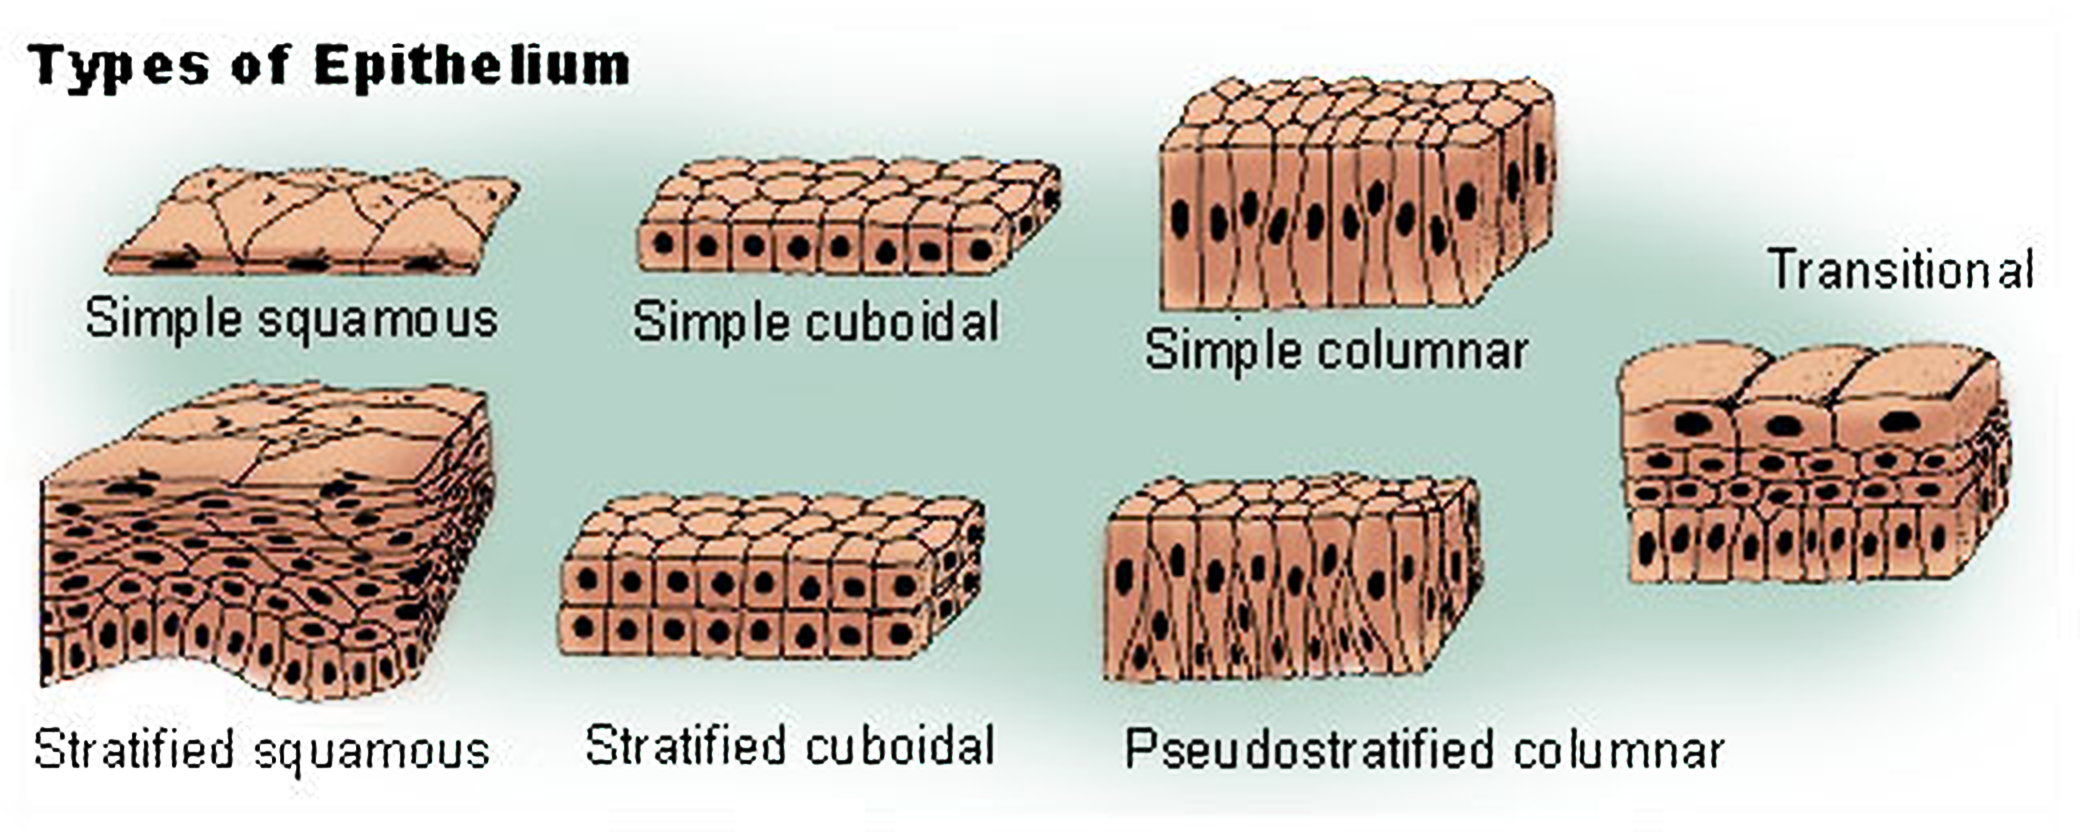
\includegraphics[width=\textwidth]{../diagrams/output.png}
\caption{The Types of Epithelial Tissue. Image credit~\cite{Epithelium}.}
\label{fig:types}
\end{figure}

As Figure~\ref{fig:types} shows, there are many types of epithelial tissue in animals which vary in their number of layers and how the cells are shaped. Each of these types of cells are found in a different region of the body where they perform a specific function.  For example, the simple squamous epithelium is no more than one layer of cells thick, and the cells are much flatter than they are wide. Because these cells are well suited to allow diffussion across themselves, simple squamous tissue is found in the walls of blood vessels and in the alveoli in the lungs, where the diffusion of oxygen occurs. On the other hand, columnar cells are much taller than they are wide, and are thus well suited to absorption. These cells are found in the intestines where they absorb nutrients from passing food. Stratified squamous epithelia are several layers thick and line the esophagus and mouth and protect against abraision.
What all of these tissues have in common, however, is how amenable they are to computational modeling. The most easily modeled tissues are simple epithelia, which typically have near-uniform height, and very little difference in appearance between their apical and basal faces. This means that the cells can easily be approximated by a two dimensional mesh in which the surfaces where two cells touch are approximated by a line. Examples of 2D epithelial tissue simulations are presented in Figure ~\ref{fig:fourgraphs}a,b. For an example of a 2D epithelial simulation on a three dimensional surface, see Figure~\ref{fig:fourgraphs}d. The 3D simulation of stratified tissue is more difficult to implement than a two dimensional model\footnote{Even a leading epithelial tissue simulator, Chaste~\cite{ChasteMain}, still does not have stable 3D modeling capabilities.}. For an example of one successful 3D model, see Figure~\ref{fig:fourgraphs}c.

\begin{figure}[h]
    \centering
    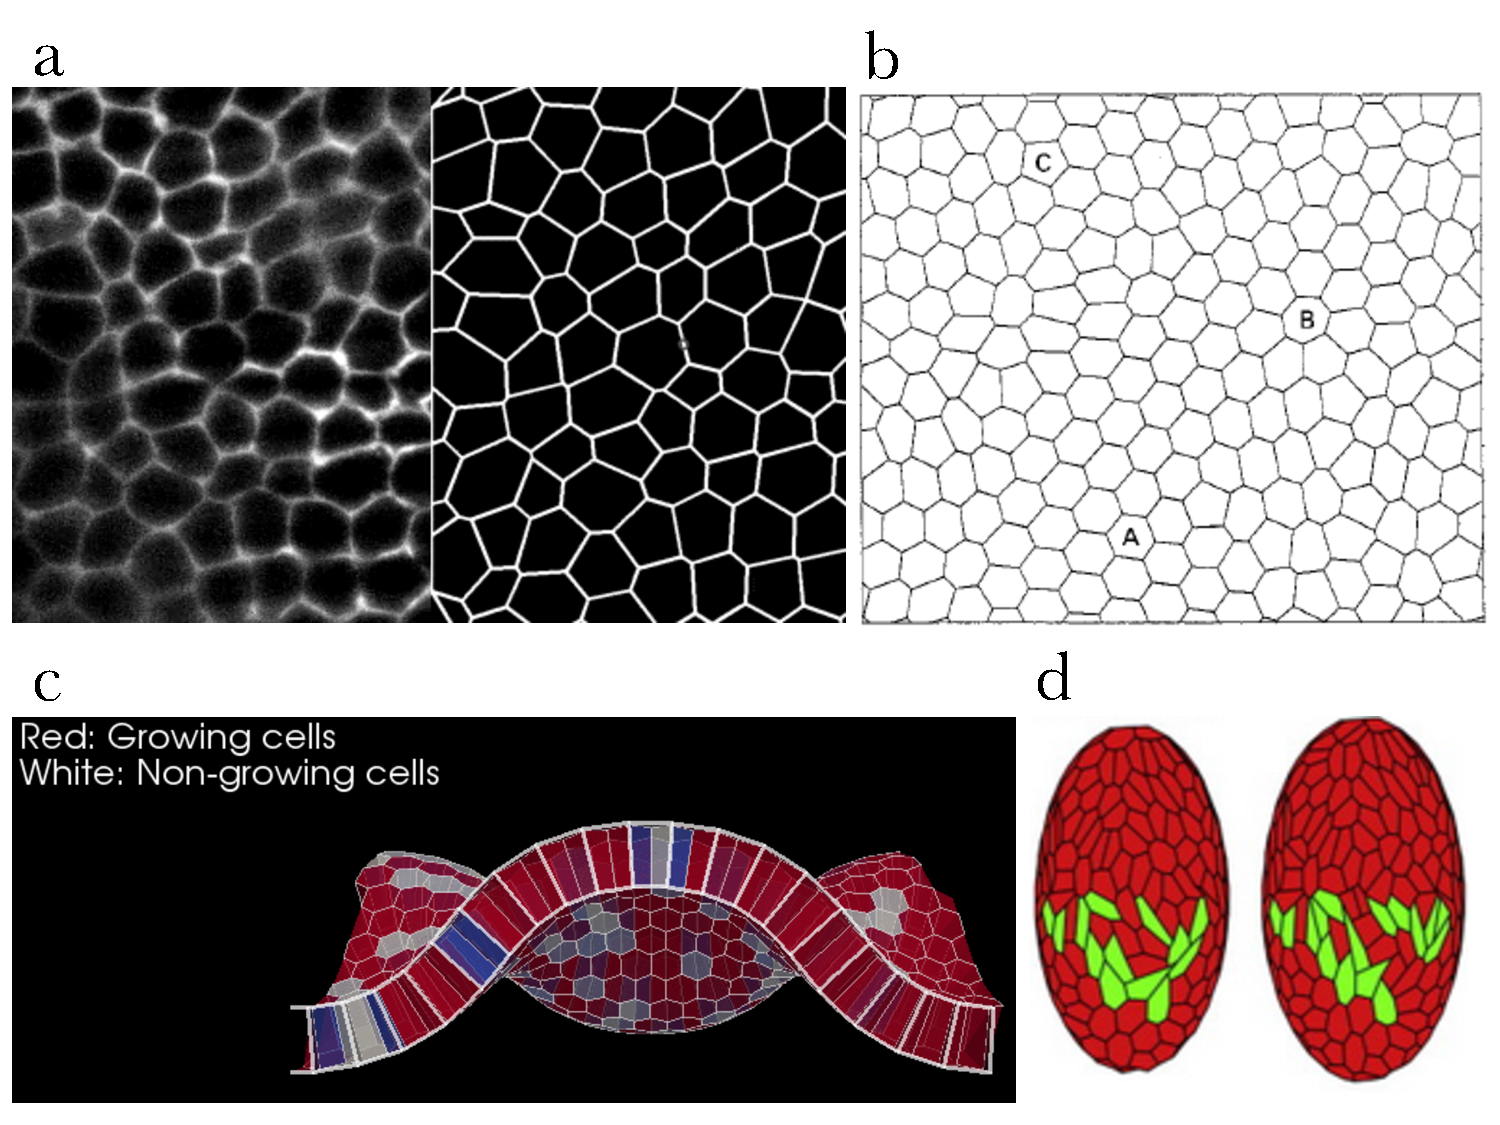
\includegraphics[width=\textwidth]{../diagrams/abcd3.pdf}
    \caption[Various Models of Epithelial Tissue]{Several screenshots illustrating the variety of epithelial tissue models. (a) A comparison of living tissue (left) to a simulation (right)~\cite{Yoshi}. (b) A diagram from the original Honda-Nagai paper~\cite{HondaNagai}. (c) A two-dimensional mesh of cells deforming in three dimensions~\cite{Okuda1}. (d) A tissue developing on a surface~\cite{VertexModels}.}
    \label{fig:fourgraphs}
\end{figure}

Current modeling is producing great results in the field of epithelial tissue morphogenisis, equilibration, and wound healing. The Honda-Nagai model, which we will discuss in great detail below, successfully reproduced the wound healing of cats' corneas~\cite{WoundHealing}. This model has also been able to reproduce all of the essential dynamics of epithelial tissue~\cite{HondaNagai}.  Current imaging tools have enabled the recording of epithelial tissue dynamics \emph{in vivo}~\cite{Sokolow, Xiong}, providing a wealth of experimental data which can serve as either initial conditions for simulations, or as benchmarks to measure the accuracy of computational predictions. In turn, models of epithelial dynamics can provide insights into the physical parameters that govern tissue development, maintenance, and malady.

Other modeling communities share advanced, free, and parallel simulation codes. For example, consider LAMMPS~\cite{LAMMPS} for simulating atomistic materials, and CHARMM~\cite{CHARMM}, Amber~\cite{Amber}, and NAMD~\cite{NAMD} for the molecular dynamics simulation of biomolecules. Unfortunately, there are only a handful of codes in use for the simulation of epithelial tissue, and to the best of our knowledge only one of them is freely available~\cite{ChasteMain}. In this thesis I will present the basic ideas of \textbf{vertex dynamics models} of epithelial tissue, and then describe the implementation of one of them as a freely available modeling tool for the community.

\section{Modeling Epithelial Tissue} 
\label{sec:modeling}

A two dimensional \textbf{vertex dynamics model} of epithelial tissue is made up of vertices and edges~\cite{DirichletDomains} which bound cells. The vertex dynamics model presupposes that the movement of cells in epithelial tissue can be approximated by the movement of edges and vertices. Some force is then proposed to guide epithelial cell movement according to an equation of motion that is solved via some numerical method.

Epithelial vertex dynamics has been a lively field of research since the 1970s because of several heartening results. Some researchers have had success modeling the morphogenesis of \emph{Drosophila} wing growth~\cite{Farhadifar}, whereas others have accurately reproduced the dynamics of corneal wound healing~\cite{WoundHealing}. In other research, simulations have faithfully captured the effects of laser perturbations to epithelial cell junctions~\cite{Yoshi}, and others have quantified parameters which are important in describing the formation of the epithelial envelope in \emph{Drosophila}~\cite{Sokolow}. Unfortunately, these results have not come from one standard model of epithelial tissue development, but from a variety of different, often irreconcilable, models. Two different approaches to epithelial simulation described below will clearly illustrate the variety of techniques in practice.

In the model developed by M. Weliky and G. Oster, forces due to osmotic pressure and contractile tension describe how vertices move~\cite{WO}. This model also allows for certain forces external to the tissue to be applied at each node. In the end, the force applied to each vertex in the mesh is given by
\begin{equation*}
F_i = F_{ext}+\sum\limits_{n=1}^N(T_{i-1}^n - T_{i+1}^n + P^n)
\end{equation*}
where $n$ is the index of the $n^{th}$ cell which touches vertex $i$. The force applied to vertex $i$ coming from cell $n$  is seen graphically in Figure~\ref{fig:WO}.
\begin{figure}[h]
\centering
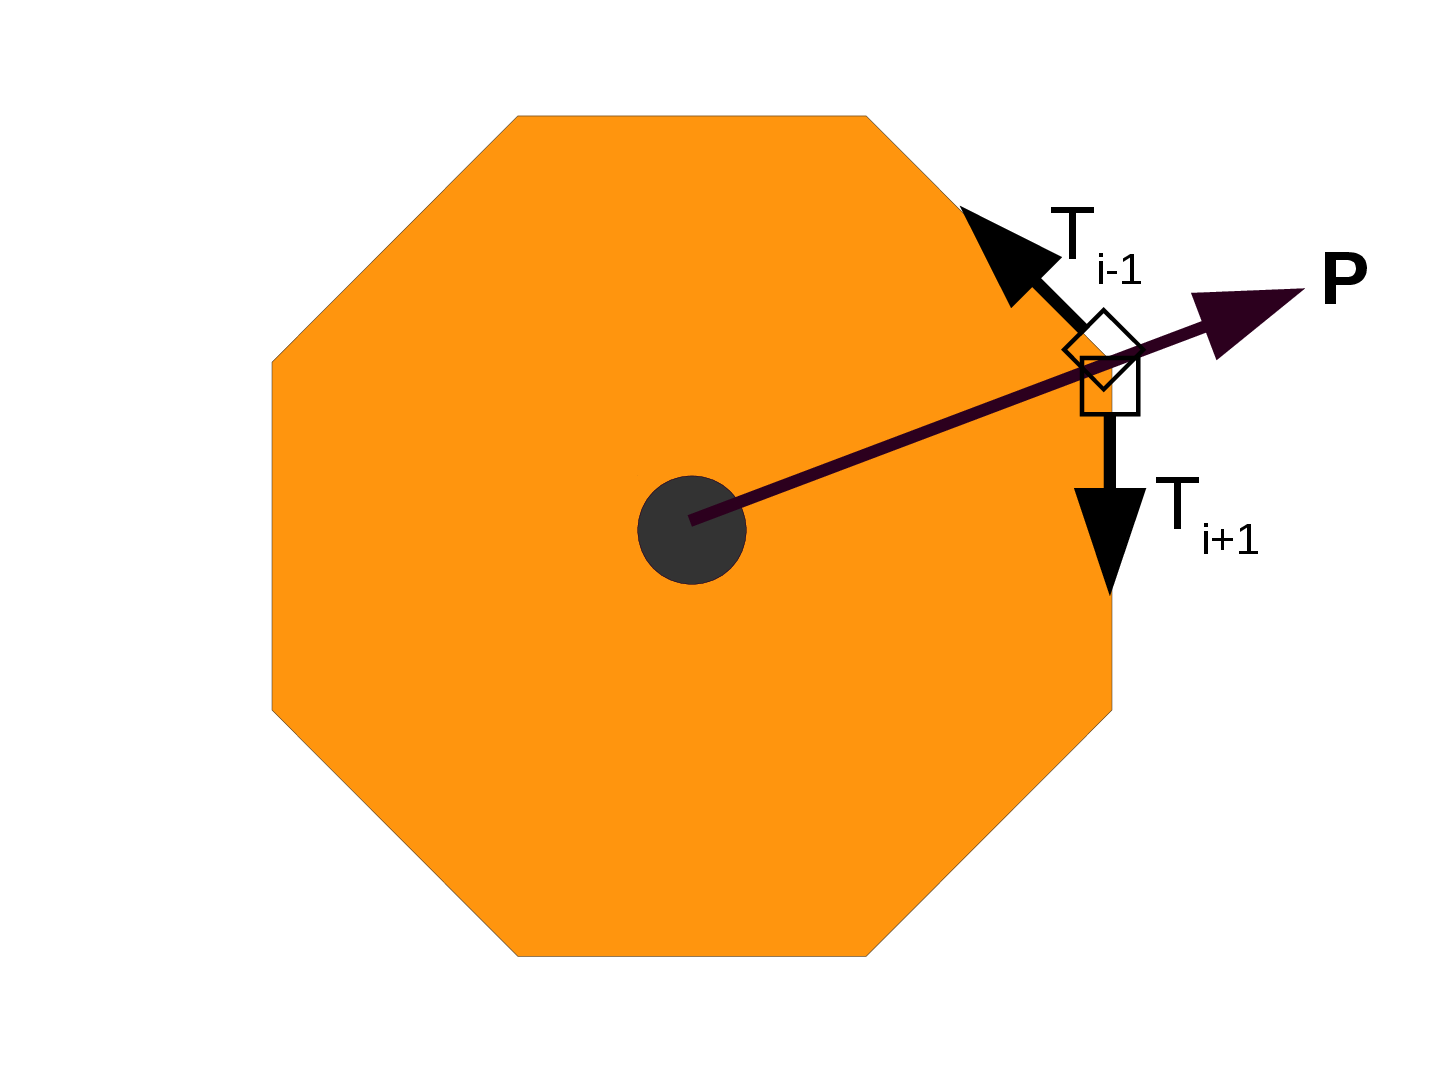
\includegraphics[width=0.5\textwidth]{../diagrams/welikyoster.png}
\caption{The Weliky-Oster Force.}
\label{fig:WO}
\end{figure}

In contrast, the model developed by H. Honda and T. Nagai takes an approach to modeling epithelial tissues rooted in the study of cellular structures\footnote{Including living and non-living. structures}~\cite{VertDyn}.  In the fantastic review paper \emph{Soap, Cells, and Statistics}~\cite{Soap}, D. Weaire and N. Rivier argue for the existence of some natural mechanism underlying the development of epithelial tissue, columnar basalt formations, soap froths, grain growths, and other cellular structures, as they exhibit a great deal of similarity. For example, consider the images of epithelial tissue presented throughout this paper juxtaposed with the image of The Giant's Causeway in Northern Ireland in Figure~\ref{fig:cause}. The equilibrium states of these structures all contain primarily hexagonal cells, and three cells typically meet at any junction. There are some differences in the exact distribution of cell shapes, the presence of chemicals in biological tissues versus the absence of growth inducing chemicals in geological structures, and the active migration of biological cells versus the entirely passive movement of soap froths; still, the authors conjecture that the dominant principle behind all cellular dynamics is the principle of maximum entropy, by which the structures seek a state with minimal potential energy.

\begin{figure}[h]
\centering
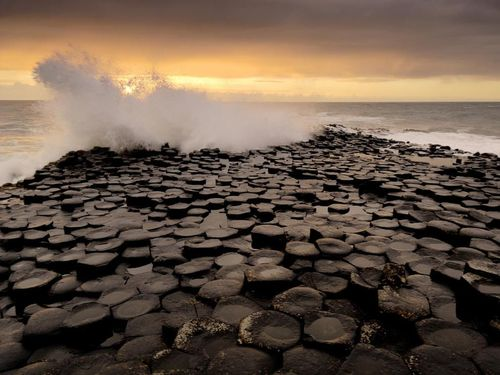
\includegraphics[width=0.5\textwidth]{../diagrams/resize_giant.jpg}
\caption{The Giant's Causeway. Adapted from~\cite{Giant}.}
\label{fig:cause}
\end{figure}

A very basic result from physics is the relationship between force and potential energy:

\begin{gather}
\vec{F} = (F_x, F_y, F_z)\\
W = -\Delta U(\vec{x}) = \int_{x_0}^xF_xdx+\int_{y_0}^yF_ydy+\int_{z_0}^zF_zdz\\
\nabla(-\Delta U(\vec{x})) = \nabla\Bigg(\int_{x_0}^xF_xdx+\int_{y_0}^yF_ydy+\int_{z_0}^zF_zdz\Bigg)\\
-\nabla U(\vec{x}) = \vec{F}
\end{gather}

In the Honda-Nagai model, the authors posit that dynamics of epithelial cell packing is dominated by their seeking a state with minimal potential energy. They describe several stores of potential energy in a tissue, take a gradient of the energy function as described above, and then apply the resulting force to the vertices in the epithelial mesh~\cite{HondaNagai}.

While both the Honda-Nagai and the Weliky-Oster models successfully reproduce the topological and geometric properties of epithelial tissue, I have chosen to focus my efforts on the Nagai-Honda model. This was the original vertex dynamics model, it still enjoys considerable use by other researchers, and is of a form quite similar to that used by others~\cite{Farhadifar}.

\section{The Nagai-Honda Model}
\label{sec:force}
\subsection{How the Vertices Move}
In 1989, K. Kawaski showed that the dynamics of grain growth can be reduced to a first order system given by:
\begin{equation}
\label{eq:motion}
\eta\frac{dr_i}{dt} = F_i
\end{equation}

where $F_i$ denotes the force applied to vertex $i$, $r_i$ denotes the position of the $i^{th}$ vertex,  and the left hand side is the velocity of the vertex multiplied by a positive drag coefficient, $\eta$~\cite{1989Kawasaki}. This is equivalent to $m_i\frac{d^2r_i}{dt^2} + \eta\frac{dr_i}{dt} = F_i$, in which the 
inertial term is considered to be much smaller than the drag term.

Based upon the notion that biological cells move in a way quite similar to high temperature crystallites\footnote{Often referred to as grain growth.}, the Honda-Nagai model has~\ref{eq:motion} as its basis. The force on the right hand side of the equation is in turn defined as the gradient of an energy function, since the model presupposes that the tendency towards a state of lower potential energy is the guiding guiding principle behind epithelial tissue equilibria. The energy function is composed of three terms which reflect the properties of biological cells.

The first two potential energy terms come from the assumption that the cell is elastic, and that the cell wants to return to a target shape. Therefore, the first two energy terms are of the harmonic form: 
\begin{equation}
C(x-x_0)^2
\end{equation}

where $x$ is some physical quantity, and $C$ is some constant. The plot of this energy is therefore a parabola with a minimum at $x =  x_0$, and the farther the quantity $x$ strays from the equilibrium, the steeper its gradient it will be, and the more forcefully it will want to return to equilibrium.

The third energy term is an adhesion energy, which is proportional to the amount of interfacial surface area between a cell and its neighbor. There is a successful theory in biology called the \textbf{differential adhesion hypothesis} which attempts to account for certain cellular distribution phenomena through their adhesive binding tendencies. The theory essentially says that certain cells tend to bond more tightly to cells of type A than to cells of type B due to the presence or absence of different adhesion proteins in the membranes of these cells ~\cite{DA}. In proliferating tissues, this difference in binding energies leads to cell segregation and the formation of structures tissues and organs. 

The precise statement of the potential energies discussed above are the following:

\begin{enumerate}
\item The deformation energy term $U_D$ is given by \\ 
\begin{equation}
U_D = \lambda(A - A_0)^2
\end{equation}
 where A is the cell area, $A_0$ is the target cell area, and $\lambda$ is some positive constant.
\item The membrane surface energy term $U_S$ is given by
\begin{equation}
U_S = \beta(P - P_0)^2
\end{equation}
 where $P$ is the cell perimiter, $P_0$ is a target perimeter, and $\beta$ is some positive constant.
\item The cell-cell adhesion energy $U_A$ is given by
\begin{equation}U_A = \displaystyle\sum\limits_{j = 1}^{n}\gamma_{j}d_{j}\end{equation}
where $n$ is the number of vertices in the cell, $\gamma$ is some constant for the boundary in question between one cell and another, and $d$ is the distance between one vertex and the next in a counter clockwise fashion. Note that in two dimensions the boundary is a distance $d$, but in three dimensions it would have to be the area of a cell face. 
\end{enumerate}

In total, the potential energy in a sheet of $N$ cells is given as:
\begin{equation*}
U = \sum\limits_{c = 1}^N\left(\lambda_c(A_c - A_{0_c})^2 + \beta_c(P_c - P_{0_c})^2 + \sum_{edges\in c}\gamma_{edge}d_{edge}\right)
\end{equation*}

 As seen in~\cite{ChasteMain}, the negative gradient of this potential energy is:

\begin{equation}
\label{eq:force}
\begin{split}
F_i = -\displaystyle\sum_{l\in N_i}(2\lambda(A_l - A_{0_l})\nabla_iA_l + 2\beta(C_l - C_{0_l})(\nabla_i d_{l, I_l-1}+\nabla_i d_{l, I_l}) +\\ \gamma_{l, I_l-1}\nabla_i d_{l, I_l-1} + \gamma_{l, I_l}\nabla_i d_{l, I_l}
\end{split}
\end{equation} 
where $l$ is the $l^{th}$ cell containing vertex $i$, given a counter clockwise orientation. $I_l$ is the local index of node $i$ in element $l$. A detailed derivation of the force follows, as in~\cite{ChasteMain}.

 The area of a convex cell made up of $n$ vertices is given by Gauss's shoelace formula:
\begin{equation}
A = \frac12\sum\limits_{i=1}^n\Big(x_iy_{(i+1)mod(n)}-x_{(i+1)mod(n)}y_i\Big)
\end{equation}
Therefore, the gradient is given by:
\begin{equation}
\nabla_i A_l = \frac12
\Big(
y_{I_l+1} - y_{I_l-1},\;\;x_{I_l-1} - x_{I_l+1}
\Big)
\end{equation}
 where the superscripts $l$ denote that x, y are in cell $l$. The subscripts are local indices in the cell $l$, and the orientation of vertices is counterclockwise. The circumference is given by:

\begin{equation}
P = \sum\limits_{j=1}^Nd_j = \sum\limits_{j=1}^N\sqrt{(x_{j+1} - x_j)^2 + (y_{j+1} - y_j)^2}
\end{equation}
Therefore
\begin{gather}
\nabla_iP = \nabla_id_{i-1} + \nabla_id_i
\end{gather}
and
\begin{equation}
\nabla_id_{l, j} = \frac1{d_{l, j}}
\Big(
x_{j+1}- x_j,\;\; y_{j+1} - y_j
\Big)
\end{equation}
Substituting the above values into the equation:
\begin{equation}
-\nabla_iU = -\nabla_i(U_D + U_S + U_A) = F_i
\end{equation}
gives the force described in equation~\ref{eq:force}.

\subsection{Topological Changes to the Mesh}
\begin{figure}
    \centering
    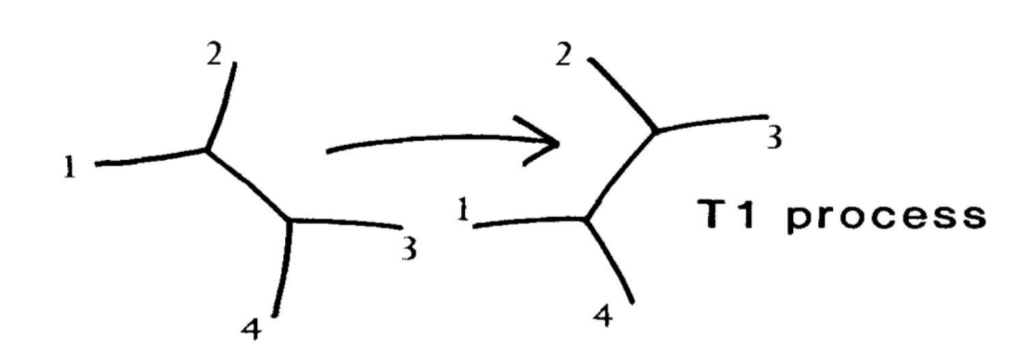
\includegraphics[width=\textwidth, keepaspectratio]{../diagrams/t1.png}
    \label{fig:t1}
    \caption[A T1 Swap]{A T1 Swap. Two neighboring cells are no longer neighbors after the swap. Adapted from~\cite{Soap}}
\end{figure}
There is emprirical evidence that nearly all vertices in a sheet of epithelial tissue have coordination number three (most vertices have three incident edges)~\cite{EpithelialTopology}. This observation has led many researchers in the field of cellular structures to consider what sort of topological changes can occur in meshes of cells without changing their connectivity~\cite{Soap}.  As it turns out there are three changes which can occur, called the T1, T2 and T3 swaps, and the original Honda-Nagai Model implements the first two.

 The T1 swap, illustrated in Figure~\ref{fig:t1}, is also called a ``neighbor exchanging swap" because two cells that were adjacent cease to be neighbors and two cells that weren't adjacent become neighbors. The T1 swap occurs when two vertices become critically close to each other, and instead of allowing the vertices to collide we rotate the offending edge. There is no specification in the literature about how to rotate the edge, but the natural choice is to turn the edge by 90 degrees. In nature this should correspond to two vertices getting very close, colliding, and then flattening out into an edge. The Honda-Nagai model performs this action discretely as a simplifying measure to avoid having to handle the momentary degree four vertex.


\begin{figure}
\centering
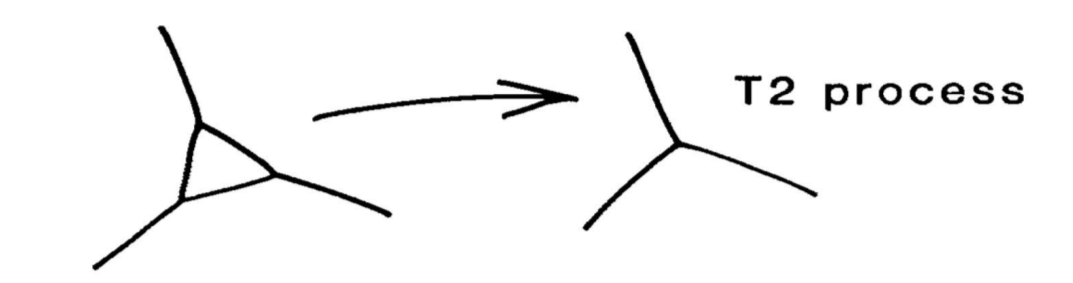
\includegraphics[width=0.5\textwidth]{../diagrams/t2.png}
\caption[A T2 Swap]{A T2 Swap. Adapted from~\cite{Soap}}
\label{fig:t2}
\end{figure}


The second topological change is the T2 swap, which is also known as ``cell removal''. A T2 swap occurs when an edge of a triangular cell becomes too small and the cell is deleted and replaced by a single vertex located at the centroid of the cell (Figure~\ref{fig:t2}).

\subsection{Selection of Parameters}
The basic vertex dynamics model requires the user to specify the $A_0$, $P_0$, and $\gamma_{edge}$ parameters for each cell, as well as a value for the drag coefficient $\eta$ and the integration timestep $dt$. The equations in this model are dimensionless. I will not undertake a discussion of how to derive the dimensionless model from the dimensional model, but for the curious reader this is all laid out in~\cite{HondaNagai}. Typically, one would not choose the values of the aforementioned parameters, but would instead have some dimensional biological data and go through the necessary conversion steps to use them in the simulation~\cite{NewOkuda}.

Interestingly, I haved found very few explicit statements of the parameters used in simulation (exceptions are~\cite{WoundHealing, ChasteMain, NewOkuda}). As Honda has said, ``We do not have accurate values for the cell parameters at present''~\cite{Honda3D}.  Very recently, new imaging techniques have permitted the \emph{in vivo} observation of epithelial tissue morphogenesis \footnote{Morphogenesis is the development of shape in an organ or organism.}~\cite{Sokolow, Xiong} and this will likely open new doors for a more accurate parameterization of current models, or perhaps even for the reformulation of the expressions for forces and potential energies. 

\begin{figure}[ht]
\centering
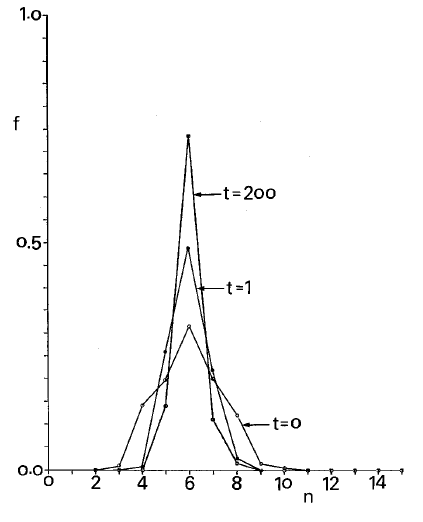
\includegraphics[width=0.5\textwidth]{../diagrams/distibutionHonda.png}
\caption[Distribution of Cell Shapes]{The distribution of cell shapes as a function of time in the original Honda-Nagai Model. Adapted from~\cite{HondaNagai}}
\label{fig:hnm}
\end{figure}

In the case of the Honda-Nagai Model, however, there is little difference between equilibrium states attributed to various parameter choices (See Chapter~\ref{chap:Epithelium}). One of the parameter-independent defining characteristics of the Honda-Nagai model is the strong tendency toward six-sided cells in equilibrium (Figure~\ref{fig:hnm}).  Yet, it has been shown that different parameter values coupled with other mesh changing operations (such as oriented cell division) can cause drastically different types of morphogenesis~\cite{Overview}. For example, drosophila wings, with their highly oriented divisions, have been shown to contain approximately 80\% hexagonal cells whereas simulations of tissues with purely stochastic divisions converge to  approximately 47\% hexagons~\cite{EpithelialTopology}. While all epithelial tissue has a strong tendency towards achieving an equilibrium dominated by hexagons, the width of the distribution of cell shapes differs by cellular structure and, hence, by parameter choices~\cite{Soap}. 


\section{Further Remarks About Epithelial Tissue Modeling}
Over the years, various modifications and improvements have been made to the Honda-Nagai model. These changes involve new ways of specifying the potential energy, adding new cell dynamics, and changing the connectivity of the mesh. In this section I will discuss some of these advances, as well as present some important mathematical theory underlying epithelial tissue models.


\begin{figure}
\centering
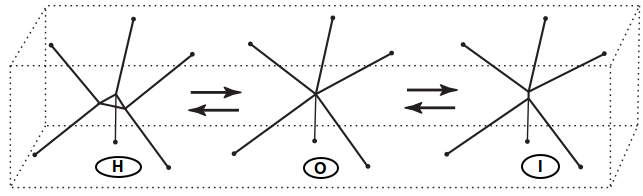
\includegraphics[width=\textwidth]{../diagrams/hoi.png}
\caption[The HOI swap.]{The HOI swap. \emph{H} configutation(left),\emph{O} configutation (center), \emph{I} configuration (right).}
\label{fig:hoi}
\end{figure}

\subsection{Three dimensional models: Honda-Nagai and Okuda.}
Honda and Nagai also implemented their model in three dimensions and used the same equation of motion for the tissue. However, while the vertices in two dimensions all meet at the junction of three edges,  in three dimensions the vertices meet where four edges are coincident, and each edge is touched by four polygonal faces. A new type of topological change handles the new connectivity, as the T1 and T2 swaps work only on two-dimensional meshes. The so-called HOI swap (Figure~\ref{fig:hoi}) looks at all of the edges in the mesh and finds the edges measuring less than $\delta$; then, it proceeds on a case by case basis. If the edge lies on a triangle, then it is of the \emph{H} form, and the swap goes from left to right (as indicated in Figure~\ref{fig:hoi}). Otherwise, the edge is of the \emph{I} form, and the transformation goes from right to left~\cite{Honda3D}. The Honda-Nagai model in three dimensions has been successful in describing how embryonic epithelial cells grow in a plane at the expense of not proliferating in the orthogonal direction, but is not the only 3D epithelial growth model.
\begin{wrapfigure}{r}{0.5\textwidth}
  \begin{center}
    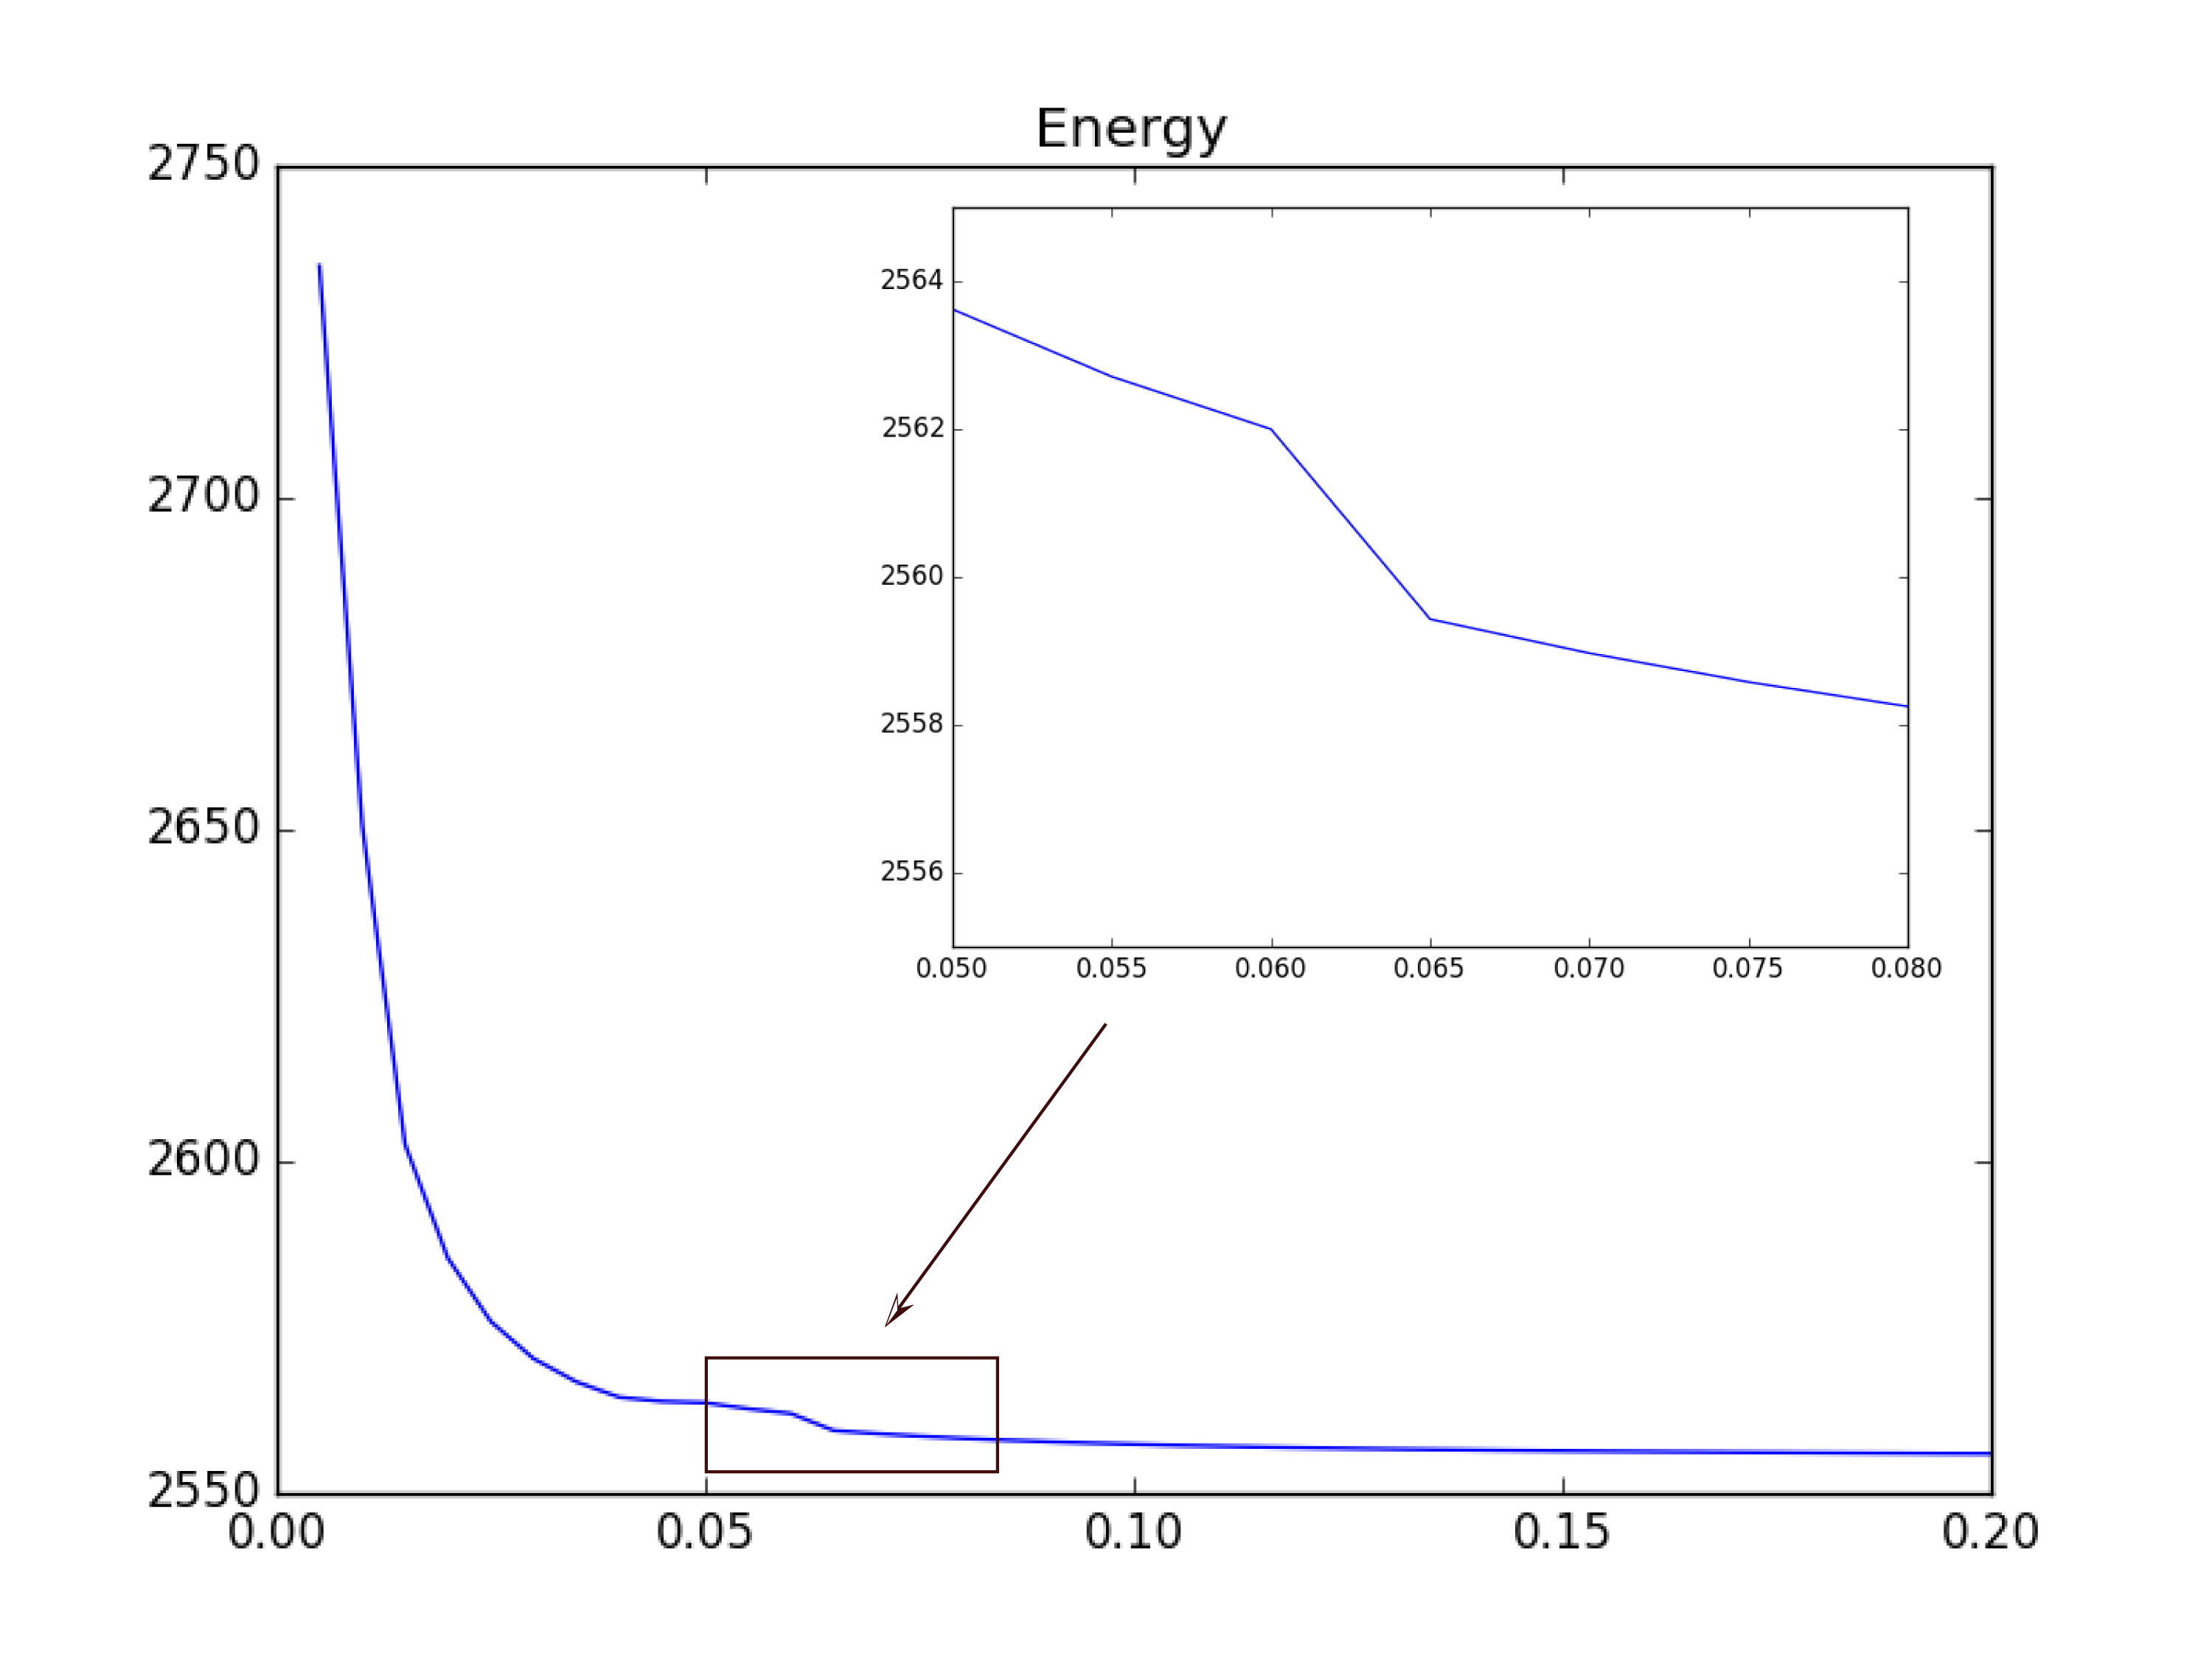
\includegraphics[width=0.48\textwidth]{../diagrams/jump.png}
  \end{center}
\caption{A jump in the potential energy. The reconnection scheme of the Honda-Nagai model can 
result in curves which are not smooth under certain circumstances.}
\label{fig:jump}
\end{wrapfigure}
The 3D vertex dynamics models recently developed by Satoru Okuda take a slightly different approach than Honda and Nagai. The Okuda models of epithelial tissue morphogenesis feature an altered cell reconnection model(Reversible Network Reconnection, or, RNR) which allows new tissue dynamics to develop~\cite{Okuda1}, and include a new viscosity term in the equation of motion which gives the model more physical plausibility~\cite{Okuda3}.

In 2012, Okuda proposed a new reconnection scheme which contrasts with the Honda-Nagai model in that there are no large inconsistencies in the energy output (Figure~\ref{fig:jump}). The principal idea behind the RNR is that a triangular element ought not be reduced to a point unless \emph{all} of its edges are critically small, whereas in the two-dimensional Honda-Nagai model a T2 swap (and in the three-dimensional model, an HIO swap) occurs when only one edge of a triangular face is smaller than $\delta$. This can lead to jumps in potential energy, as well as generate artifical tissue dynamics which only occur because edges which are larger than the approximated zero length ($\delta$) are forced to zero. Due to the fact that a triangle is forced to a vertex, the occurence of an oscillation through several T2/HOI swaps at a vertex is not seen by the model. The two drawbacks to the RNR model are that it may not produce quality results when simulating tissues in which topological irreversibility is a defining feature~\cite{CellSurf}, and that the model can sometimes produce topologies which are not computable by the software implementing it (i.e. when one edge of a triangle becomes critically small, while the other two remain long, and the triangle becomes a double edge between two vertices~\cite{Okuda3}).

Okuda's other innovation was the introduction of a new viscosity term into the equation of motion for a vertex, giving:
\begin{equation}
F_i = \eta_i(\frac{dr_i}{dt} - \vec{v_i})
\end{equation}
where the $v_i$ is a vector which describes the viscous force acting on a vertex as a result of its local interactions with neighboring vertices. Observations of growing tissues show that the viscosity of a growing tissue is inhomogeneous and depends upon the cells the types of cells in a region as well as the membranes interacting with the cells, yet the vertex models existing before Okuda's did not take this into account. For this reason, the Honda-Nagai 3D model was unable to capture the morphogenetic dynamics seen in~\cite{Mao}, while the Okuda model was.


\subsection{Similar Models of Potential Energy}
Interestingly, as mentioned in section~\ref{sec:modeling}, the Honda-Nagai form for the energy in a vertex is quite similar to the form developed by Farhadifar~\cite{Farhadifar}. The Farhadifar formulation is:
\begin{equation}
E_i = \sum\limits_{cells}\frac K2(A - A_0)^2 + \sum\limits_{edge}\gamma_{edge}d_{edge} + \sum\limits_{\alpha}\frac\beta2P_\alpha^2
\end{equation}

Remember the formulation of the Honda-Nagai energy:
\begin{equation*}
U = \sum\limits_{cells}\left(\lambda(A_c - A_{0_c})^2 + \beta(P_c - P_{0_c})^2 + \sum_{edges_c}\gamma_{edge}d_{edge}\right)
\end{equation*}

The equations are nearly identical, except that the Farhadifar model asserts that the cell perimeter persistently tries to collapse the cell($P_0=0$), while the potential energy due internal pressure ($A_0\ne0$) resists this tendency. Nevertheless, the topological results of this model are not wildly different from the Honda-Nagai results~\cite{Farhadifar}.

\subsection{The T3 Swap}
The T3 swap is also known as ``mitosis'' or ``cell division''. Cell division was not a part of the original Honda-Nagai Model~\cite{HondaNagai} that dealt with the equilibration of a fixed number of cells. However, during proliferation cells divide, and computational models need to take into account tissues with varying numbers of cells. The challenge with implementing the T3 swap is that there are infinitely (within the bounds of floating point arithmetic) many choices about where to divide a cell, and there are several competing opinions (though no unanimouslly accepted theory) about how the dvision is oriented. Some cells divide along their longer axis, which is known as the `Hertwig's Long Axis Rule', but global tissue stress and local cell geometry are also thought to affect the orientation of mitosis~\cite{Order, Orientation}. The computational realization of a T3 swap is trivial, as the swap occurs by placing two new vertices along the edges of a cell and joining them by a new edge. The trouble is that there is no specification about which edges ought to have vertices implanted, or where to insert these vertices. The choice of where to divide a cell in a proliferating tissue can have profound effects upon the geometric appearance of a tissue - indeed, improperly oriented cell divisions are an indicator of cancer~\cite{EpithelialTopology, misaligned}. 
\begin{figure}
\centering
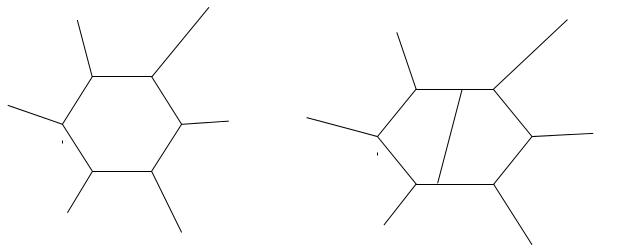
\includegraphics[width=\textwidth]{../diagrams/t3.png}
\caption[The T3 Swap.]{The T3 Swap. Adapted from~\cite{Soap}.}
\label{fig:t3}
\end{figure}

\subsection{The Euler Characteristic and Its Implications}
The majority or current vertex dynamics models assume that all vertices have a coordination number of 3, since empirical evidence shows that the vast majority of cells have this property~\cite{EpithelialTopology,Overview}. In this section I will expand upon some observations made in~\cite{Soap} that deal with this phenomenon. \textbf{Euler's Formula} is an equation which relates the number of edges, faces, and vertices in a graph or polyhedron. An invariant $\chi$ relates the faces, edges, and vertices as follows:

\begin{equation}
\chi = V - F + E
\end{equation}

The invariant depends upon the graph or polyhedron in question. We will ignore the exact value of $\chi$ and simply use the fact that it is a constant. We know that each vertex connects to exactly three other vertices. Then we notice that all edges have two vertices, and that all vertices are connected to three edges. Inititally, our intuition tells us that there should be three times as many edges as vertices, which leads us to the incorrect formula:
\begin{equation}
3V = E
\end{equation}
But then we notice that if we consider all of the vertices in the mesh, we count each edge twice, so we divide by two and then simplify to get:
\begin{equation}
3V = 2E
\end{equation}

Similarly, if we consider how to relate the number of edges to the faces in the mesh, we conjecture that the number of edges in the mesh is equal to the sum of the products of cell shapes by the sides, $k$,  per shape. More clearly, we might guess the following:
\begin{equation}
\sum_{k=3}^N kF_k = E
\end{equation}
Where $N$ is the highest number of edges in any cell in the mesh. But in this way we have again counted all of the edges twice, so the true number of edges must be the summation above divided by 2. We simplify the equation to get
\begin{equation}
\sum_{k=3}^N kF_k = 2E
\end{equation}
Now, we are able to reduce Euler's Formula to one variable using the relationships given above.
\begin{gather}
V - F + E = \chi\\
\frac{2E}3 - F + E = \chi\\
\frac{5E}3 - F = \chi\\
\frac{\sum_{k=3}^N kF_k}{6} - F = \chi\\
(\frac{\sum_{k=3}^N kF_k}{F} - 6)F = 6\chi
\end{gather}

Biological cells are very small, and an epithelial tissue is composed of many cells, so we assume that $F\to\infty$ and then immediately notice that the expression in parentheses must tend to zero as $F$ goes to infinity, or else the left hand side of the above equation will not approach the constant $6\chi$. From here it is easy to see that the introduction of a finite number of vertices with coordination number higher than three will not affect this result in the limiting case.

So we know that the algebraic mean of the number of vertices per face must be 6. Of course we have no reason at this point to assume that there is even one cell in the mesh with exactly six edges. It is feasible that the tissue is entirely be made up of five and seven sided cells. Nevertheless, empirical evidence shows a strong central tendency in the distribution of cell shapes. Whenever a cell tries to stray from the average, there are computational means (such as the T3 swap) of recentering the distribution at 6 sides.

The choice to impose degree three on each vertex is not one hundred percent consistent with nature, but has been a part of most models of epithelial tissue.  It is a simplifying assumption that \emph{rosettes} (epithelial cells organized radially about one vertex which has degree greater than or equal to 4) do not change the global dynamics of the development of an epithelial tissue.  Recent computer vision developments~\cite{rose} have made it easier to detect rosettes in epithelial tissue samples and may in the future provide information about the number of these formations, or evidence that rosettes are an important feature of epithelial tissue. Models would need to be revised to handle the introduction of vertices of higher degree.


\chapter{Epithelium}

\section{About Epithelium}
Here I present my implementation of the Honda-Nagai Model for epithelial tissue development as the simulation software called \emph{Epithelium}. The software is easy to install, takes up less than 50Mb, comes in parallel and non-parallel versions (Version 2.0.0, Version 1.0.0) and has very few dependencies. \emph{Epithelium} allows users to specify all parameters of interest in easily modifiable text configuration files, can handle simulations of arbitrarily large size, and can generate data for animations of epithelial tissue development as well as useful plots of important variables. 
\begin{figure}
\centering
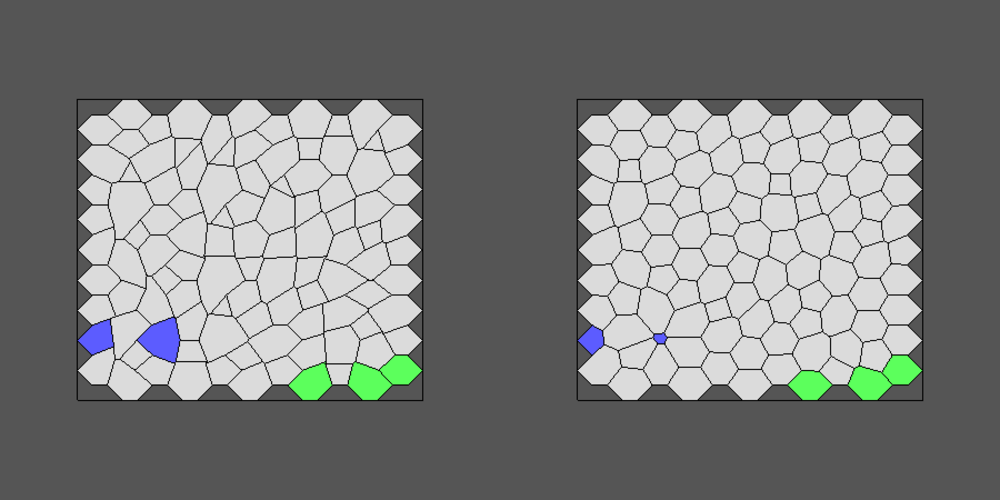
\includegraphics[width=\textwidth]{../diagrams/BeforeAfter.png}
\caption{Cells before (left) and after (right) the application of force.}
\label{fig:beforeafter}
\end{figure}
The source code is highly modularized and allows for ambitious users to easily extend the code to meet their needs. For example, alternate numerical integrators can easily replace the existing one, new mesh generators can replace the square mesh I have developed, and all data is output in space-separated formats which users with scripting language experience can transform to serve as input into the graphical utilities of their choice. In addition, the cell and coordinate classes are well documented and can be extended to output new data, as users may need. Figure~\ref{fig:beforeafter} provides a taste of the what the most basic installation of \emph{Epithlium} can do, showing a mesh of cells before and after equilibration.

\section{Sample Configuration Files}
The typical user will not want to modify source code, but would prefer to have a simple interface for changing simulation parameters. In this section we will explore in depth what the user interface looks like in terms of the three main configuration files, \texttt{config.txt}, \texttt{parameters.txt} and \texttt{change\_mesh.txt}.
\subsection{config.txt}
In this file, the user an specify some global properties about the mesh, and some important quantities for how the simulation will proceed. Most of the quantities are self explanatory. The \texttt{dimension} of the mesh refers to the number of cells along a given axis in a square mesh, and the \texttt{swap length} , \texttt{upper bound}, and \texttt{max swaps} parameters are used for performing random transformations to the mesh in the beginning of the simulation. The \textt{swap length} is the edge length below which a swap is performed. The \texttt{max swaps} parameter is the maximum nuber of random perturbations the code will make to the mesh before starting the simulation. The \texttt{upper bound} is an integer which is upper bound of the range for a random number generator. A random number generator produces a number in the range [1:\textt{upper bound}], and a random T1 swap is performed on `1'. The \texttt{delta} parameter specifies how close too vertices must be to force a T1 swap to occur.

OFF is the file format given to the plotting program \textbf{geomview} to plot the mesh. You can specify how often the code prints an image with the \texttt{frequency} parameter, but it must be a multiple of ten. More closely spaced images can be generated by using a smaller integration step size.
\begin{lstlisting}
13 # Dimension of mesh MUST BE ODD!!!!
0.01 # Maximum step size
1000 # Number of iterations
10 # frequency of OFF file output. Must be a multiple 10!
.1 # delta minimum vertex separation.
1000 # max swaps
1.5 # swap length
2 # upper bound random number generator
1 # Make energy and shape plots?
1 # Make a movie in the end? [1/0]
\end{lstlisting}

\subsection{parameters.txt}
In the \texttt{parameters.txt} file, the user can specify the parameters discussed in Chapter~\ref{chap:intro}. These are the default parameters for all of the cells in the tissue. 
\begin{lstlisting}
beta = 3;
lambda = 55;
t_gamma = 1;
t_area = 4.0;
\end{lstlisting}

\subsection{change\_mesh.txt}
While the parameters file allows global control of the mesh, the \texttt{change\_mesh.txt} file alows users to change local properties of the mesh. The first line of the file is for specifying how many $\gamma$, $A_0$, $\lambda$, and $\beta$ modifications will be made to the mesh. Note that $P_0$ cannot be changed, as $P_0$ is a function of $A_0$ (See Chapter~\ref{chap:intro}). The subsequent lines are for specifying the index and new value for each one of these modifications. As can be seen in Figure~\ref{fig:beforeafter}, cells can be color coded by parameter value to show these changes to the default settings.
\begin{lstlisting}
2 3 1 1 # num gamma, num area, num lambda, num beta
16 4.0  # gamma
17 5.1  # gamma
3 1.0   # area
4 1.0   # area
10 3.7  # area
1 10    # lambda
90 100  # beta
\end{lstlisting}

\section{Image Gallery}
Model parameters are easy to change in \emph{Epithelium}, and a variety of simulations are possible with very minimal effort on part of the user. Figure~\ref{figAFIHAoIHGa} - Figure~\ref{fig:aAIHgIASg} show the output from \emph{Epithelium} for several parameterizations. Each of the plots that follow show the decreasing energy in the mesh over time, the equilibrium distribution of cell areas, perimeters, and shapes. You may notice that there is very little variation between the plots - this is an essential property of the Honda-Nagai Model~\cite{HondaNagai} that the introduction of cell proliferation and an unbounded mesh could change.  

INSERT FIGURES

\section{The Design of \emph{Epithelium}}
The technical details of how a vertex dynamics model can be effectively implemented are not explained in great depth in the literature\footnote{\cite{ChasteMain} is an exception, but is rather advanced}. I will fill the void in this field in the section that follows and present a detailed look at the data structures and algorithms needed for the programming of the Honda-Nagai Model. It is fitting to start with a very high-level overview of the structure of the code.

\subsection{[Highly Simplified] Pseudocode}
Here I will briefly outline how the code works. All of the functions are explained in some detail later in this chapter.
\begin{lstlisting}
mesh_variables <- read_configs()
mesh <- make_mesh()
random_alterations(mesh)
copy(mesh, rotate_mesh)
rotate(rotate_mesh)
print(simulation_info) # So the user can verify all parameters.
for i = 1:num_iters
   if(iter%print_freq == 0)
      print(OFF_file)
   temp_mesh = NagaiHondaForce(mesh) 
   temp_rotate_mesh = NagaiHondaForce(rotate_mesh)
   mesh <- mesh + temp_mesh
   rotate_mesh <- rotate_mesh + temp_rotate_mesh
   performT2(mesh)
   performT1(mesh)
   performT2(temp_rotate_mesh)
   performT1(rotate_mesh)
rotate_back(rotate_mesh)
compare_mesh(mesh, rotate_mesh)
print(graphics and error analysis)
\end{lstlisting}

\subsection{Classes}
\emph{Epithelium} has a partially object oriented design. The cell and vertex classes organize the data into meaningul pieces.
\begin{itemize}
\item The {\color{red} Cell} class contains a number of useful functions and data members to make the code easy to read and understand. All cell information could have been stored in arrays, but the OO structure makes the code more readable. All cells know their index, which vertices (coordinates) make them up, they are able to calulate their area and perimeter, can modify their constituent vertices, can tell you whether or not ther contain a vertex, and can print out a graphical, color coded representation of themselves to an OFF file. Cells have other 
\begin{lstlisting}
public:
 cell(int index, vector$<$int$>$ AssociatedVertices,\
       double target_area = t_area, double gamma = t_gamma)
 {	
   assert(index $>$= 0);
   m_AssociatedVertices = AssociatedVertices;
   m_index = index;
   m_target_area = target_area;
   m_target_perimeter = sqrt(pi * m_target_area);
   m_gamma = gamma; 
 }
	
 cell(){} // Default constructor
	
 vector<int>GetVertices(){return m_AssociatedVertices;};
 int GetIndex(){return m_index;};
 void SetIndex(int index){m_index = index;};
 void SetTargetArea(double area){m_target_area = area;};
 double GetTargetArea(){return m_target_area;};
 double GetTargetPerimeter(){return m_target_perimeter;};
 double ComputeArea(double * X, double * Y);
 double ComputePerimeter(double * X, double * Y);
 void PrintCell(ofstream &OffFile);
 int ContainsVertex(int index);
 void SetGamma(double gamma){m_gamma = gamma;};
 double GetGamma(){return m_gamma;};
 void InsertVert(int v1, int v2);
 void EraseVert(int index)
 {
   vector<int>::iterator it = find(m_AssociatedVertices, index); 
   m_AssociatedVertices.erase(it);
 };
 void ReplaceVert(int before, int after)
 {
   vector<int>::iterator it = find(m_AssociatedVertices, before); 
   *it = after;
 };
 void SetVertices(vector<int> vertices)
 {
   m_AssociatedVertices = vertices;
 };
 int GetNumSides(){return m_AssociatedVertices.size();};
private:
 vector<int> m_AssociatedVertices; // Stored counterclockwise
 int m_index;	
 double m_target_area;
 double m_target_perimeter;
 double m_gamma;
};

\end{lstlisting}

\item{The Vertex Class}
The {\color{green} Vertex} class stores the index of a vertex, and 
whether or not the vertex will move during the integration. While a 
vertex object does not store the location of the vertex, it tells the 
simulator whether or not a vertex is on the border of a mesh and, if it 
is not, it is allowed to move. It was a design choice that 
\emph{Epithelium} be able to run three popular types of meshes, those 
with border, those without, and those that cover a surface.  Another 
benefit of the vertex class is that is allows users to easily extend 
the code to include forces acting on individual vertices, and to 
specify other types of vertices besides interior and exterior. The 
vertex class could be extended to include a member function such as 
activeMigration(), or any number of interesting functions. This code was developed with eyes to the future. 
\begin{lstlisting}
class vertex
{
public:
  vertex(int idx, bool t) : index(idx), IsInner(t){};
  vertex(){index = -1; IsInner = 0;};
  int index;
  bool IsInner;
  inline bool operator==(const vertex& rhs)
  {return index == rhs.index;};
};
\end{lstlisting}
\end{itemize}


\section{A Relational Database}
There is one other major idea behind the design of \emph{Epithelium}. A 
popular way to store data since the 1970's is to store data in groups of tables which are connected via \emph{keys}. This type of database is popular for reasons which will become apparent by means of a simple example. 

Consider a business which sells a number of products, and wants to keep 
track of their customers, the customer's orders, the customer's 
addresses, and information about the products ordered. A wasteful way 
to store this data is to create a large table in which the first column 
is for customer names. Next to every customer's name is the customer's 
address, and next to the customers address is the customer's order 
number. Next to the customer's order number is an item in that order, 
and next to each item ordered is the item information. This method of 
storing data is terribly redundant, because for each order with more 
than one item you would have redundant storage of the orderid, and of 
the customer information. Furthermore, every time the same item is 
order 

A better idea is to break this data up into several tables which 
together define a \emph{schema}. In the preceding example, the following tables define a good schema:
\begin{figure}
\centering
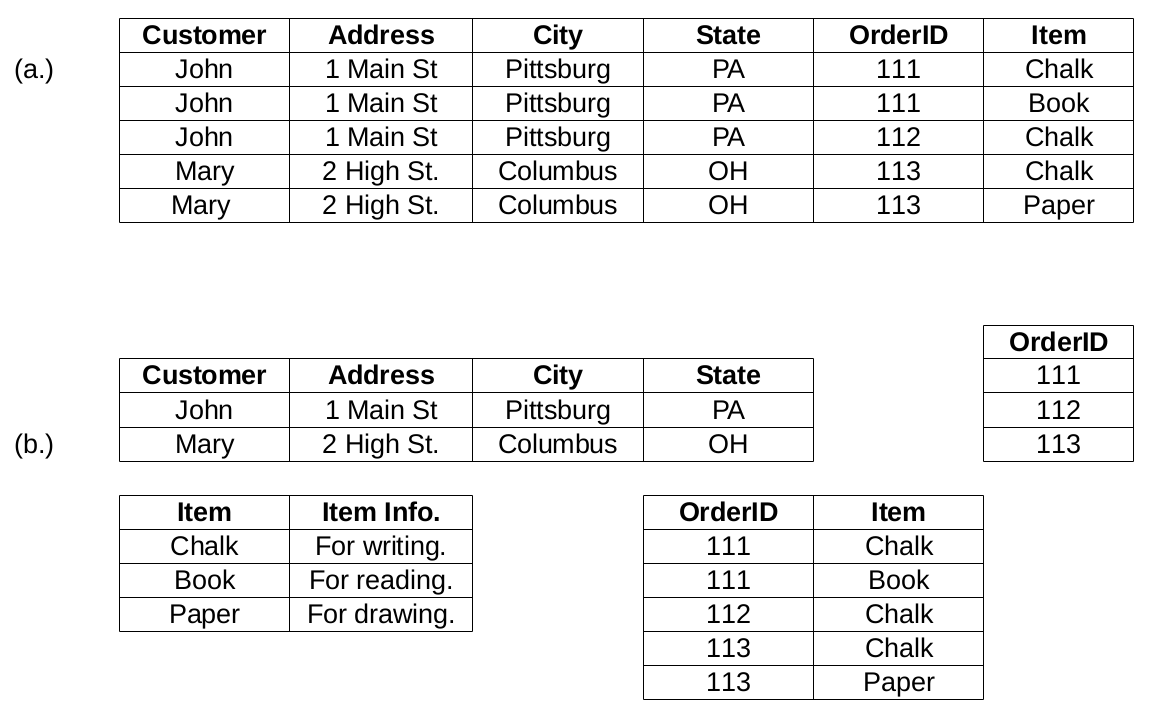
\includegraphics[width=\textwidth]{../diagrams/relationaldb.png}
\caption{An example of a relational database.}
\label{fig:rdb}
\end{figure}


We are now guaranteed that the customer information is not duplicated for every item in an order, and that item information is not duplicated every time an item is in an order.

\begin{figure}[h]
\centering
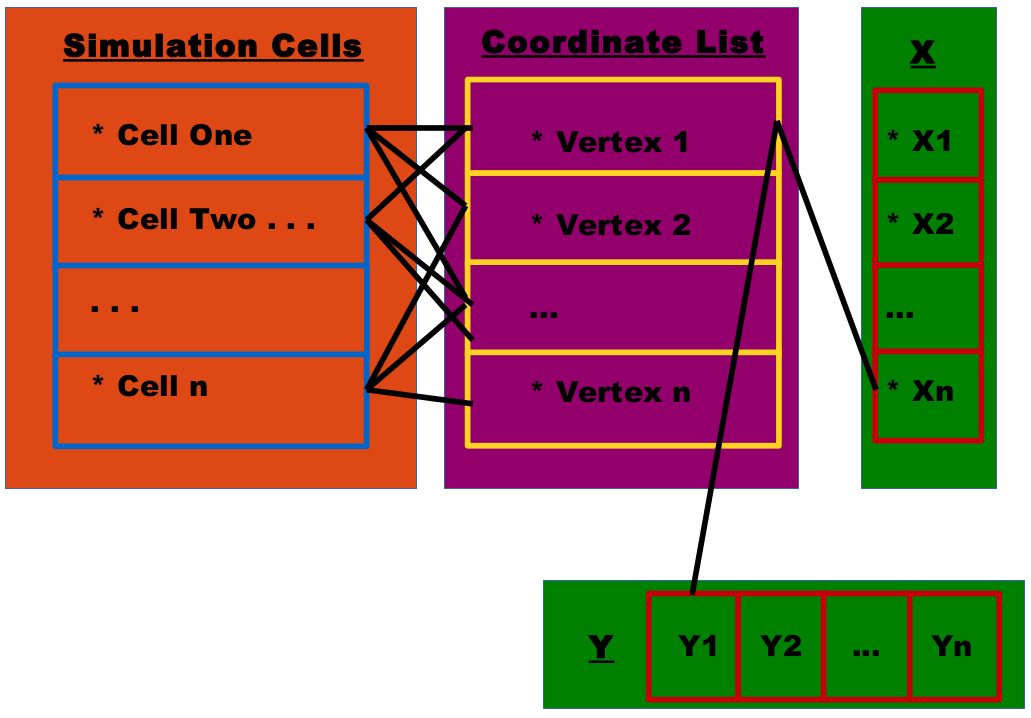
\includegraphics[width=0.5\textwidth]{../diagrams/ds.png}
\caption{\textbf{The Relational Database.}}
\end{figure}

My data structure is inspired by the relational database model. I have six tables, including the simulationCells, coordinateList, X, Y, tempX and tempY tables. The cell and coordinate tables are implemented as 1d vectors of cell and coordinate indices, whereas the position tables are implemented as 1d arrays for ease of passing these structures to CUDA C functions (will talk more about CUDA C later). The cells can extract coordinate information from the coordinateList table via the \emph{index} key, and the coordinateList can access the position information from the X and Y arrays via their own \emph{index}. The temporary X and Y arrays store temporary position information about the vertices before the mesh positions are updated. This choice saves memory because the cells, coordinates, and coordinate locations are stored independently of each other, and there is no data redundancy. 

\section{Initial Mesh Design}
The hex\_mesh() function generates an $n$x$n$ mesh of cells, where the 
dimension represents the number of cells touching the boundary in 
either axial direction. Figure ~\ref{fig:mesh} shows the default mesh 
used by \emph{Epithelium}, with the cell ids and vertex indices are 
labelled. After a sheet of cells is generated by 
hex\_mesh(), the tissue is perturbed in by first performing random 
T1 swaps on edges of the mesh, and then by perturbing the locations of a select 
number of vertices.

\begin{figure}
\centering
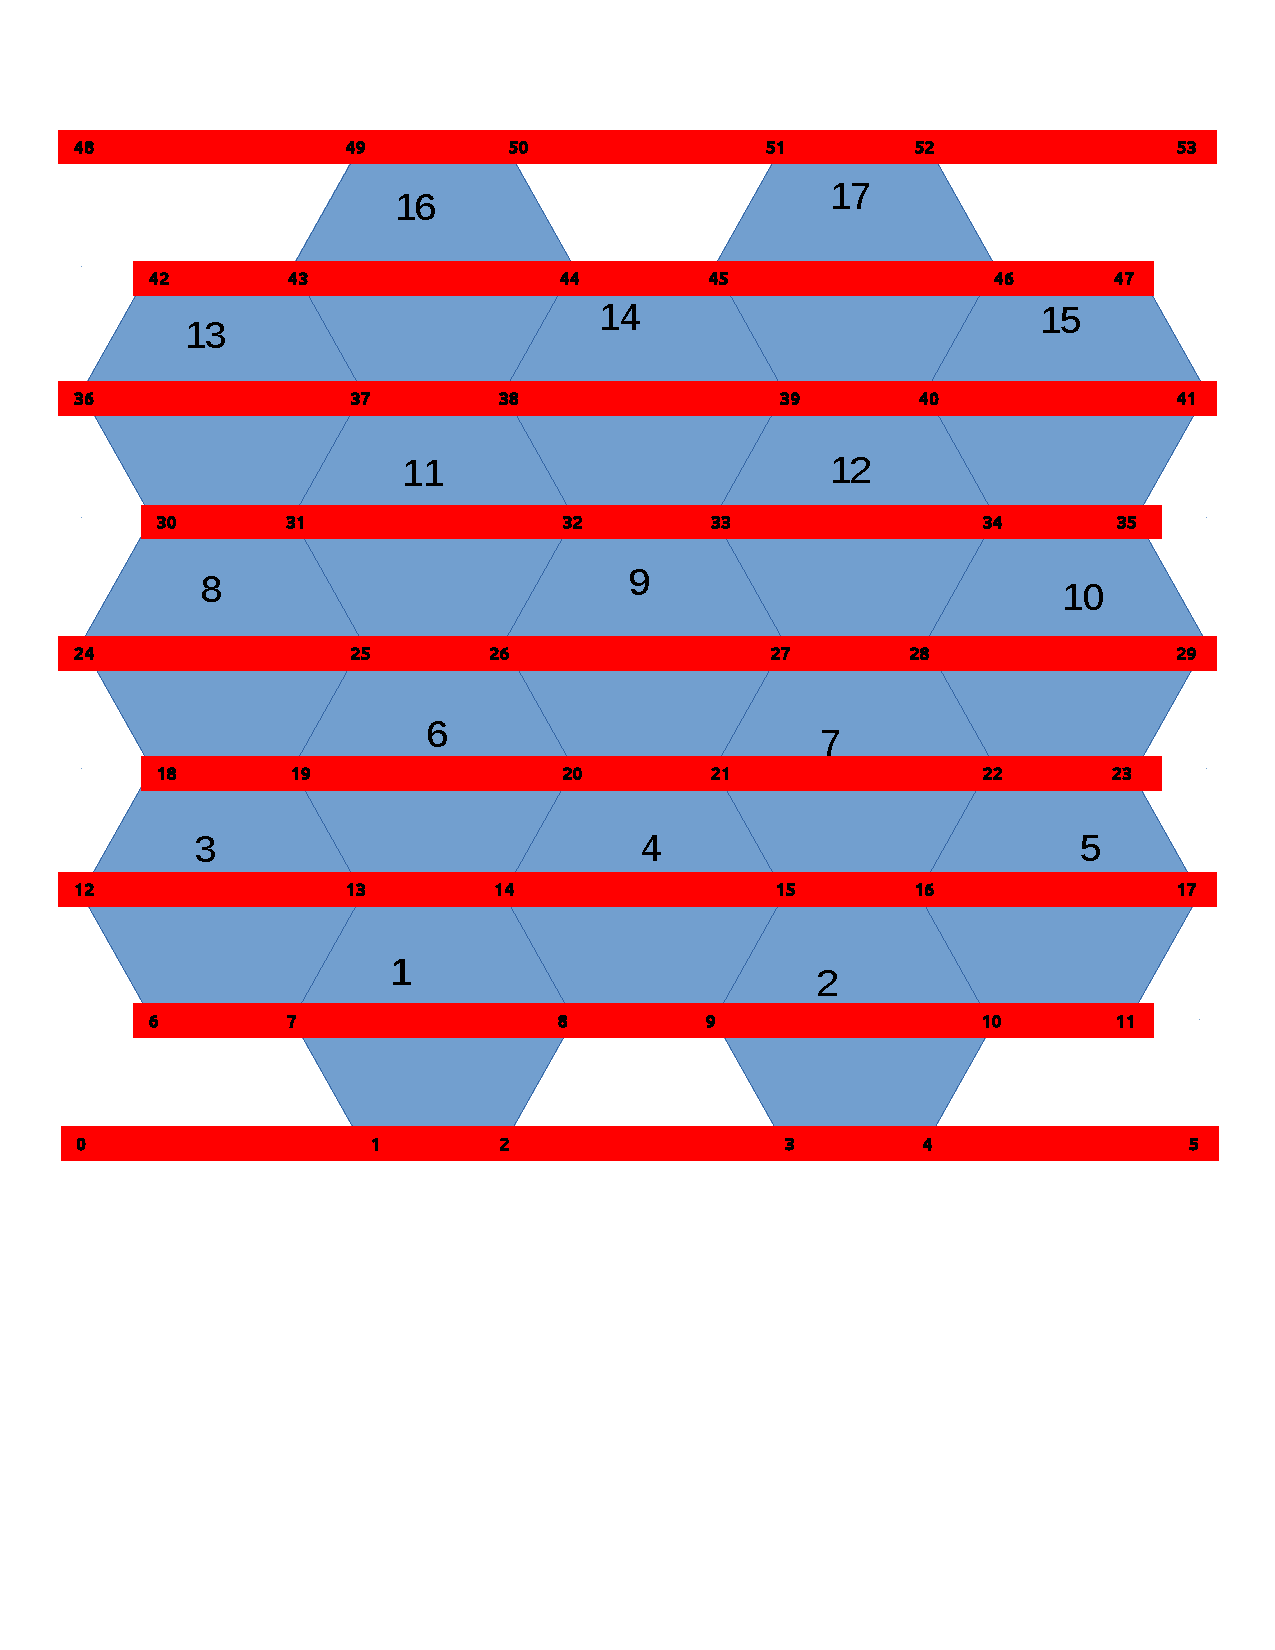
\includegraphics[height=0.7\textheight]{../diagrams/vert_mesh.pdf}
\caption[A 5x5 Hexagonal Mesh.]{\textbf{A 5x5 hexagonal mesh. The cell 
indices are written in the cells and the vertex indices are written on the red bars.}}
\label{fig:mesh}
\end{figure}
\section{Moving the Vertices}
\emph{Epithelium} loops over the vertices, computes the force applied to each vertex and then computes a displacement due to the force using the Euler Method. In their original paper, H. Honda and T. Nagai described the use of a Modified Runge Kutta Method to move the vertices, but this method would result in extra unnecessary computations at each time step. The \emph{Error Tolerance} section of this chapter describes how the Euler Method is numerically stable enough for this application. The same decision to use then Euler Method was made by the research group at Oxford that developed CHASTE, the \emph{other} leading software for implementing the Nagai-Honda Model. 

A displacement is calculated and stored in the temporary X and Y arrays. No vertex is permitted to move more than one half of the minimum delta separating vertices (the $\delta$ under which a T1 swap will occur) during an integration. By imposing this restiction we are ensuring that we will not miss the event of two vertices coming critcally close and a T1 swap occurring. Also, this prevents vertices from passing each other and invalidating the mesh. To ensure that no vertex moves too much, we store verify each displacement as we put it in the temporary X and Y arrays. If a displacement is too large, then the entire array of temporary displacements is erased, the time step is halved, and we begin the integration again. We could label the integrator as `fault tolerant'.

\begin{wrapfigure}{L}{0.4\textwidth}
\begin{center}
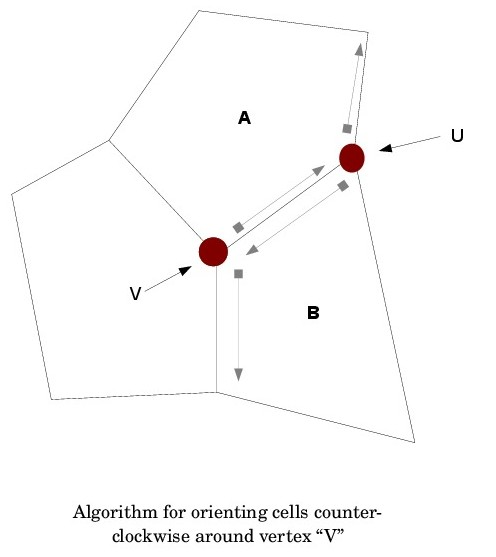
\includegraphics[width=0.38\textwidth]{../diagrams/counterclockwise.jpg}
\end{center}
\caption{Getting Cells in Order}
\label{fig:ctrclockwise}
\end{wrapfigure}

Another important aspect of the numerical integration is that cell and vertex information must be processed in counterclockwise order. In Figure~\ref{fig:ctrclockwise} I illustrate how a vertex can find the cells surrounding it in this order. When we are integrating a vertex $i$, the vertex first searches in the cell vector for a cell which contains it, and then the vertex finds the next vertex in that cell. Then, we have an edge. Some other cell contains that edge if it contains both of the vertices. That cell must be clockwise from the first. The cells are stored in the reverse order of which they are uncovered by this algorithm before the integration starts. This is a very expensive step ($O(n^3)$) in the computation, and ought to be optimized.


\section{Embarassing Parallelism and CUDA}
The numerical integrations and the vertex location updates exhibit what Cleve Moler describes as ``embarassing parallelism''. Computing the displacement of vertex \emph{a} does not depend upon the computation of the displacement of vertex \emph{b} during a given time step. Similarly, the vertex locations can all be updated in parallel since the update is simply a vector sum operation of the X and Y arrays with the temporary X and Y arrays, respectively. 

A popular hardware choice for parallel programming in last decade has been the NVIDIA GPU. CUDA is the NVIDIA extension of the C programming language which can run certain parts of C code on the GPU, while still running the serial and i/o operation on the CPU. I wrote some parts of the code in this language, and these parts were very simple to implement. The GPU is a collection of small processors, and the vertices are small, simple objects, so I mapped each vertex in the mesh to one of the hundreds of small processors to get some computational speedup.

Specifically, CUDA was employed to update vertex locations, since the sum of 1d arrays is well suited to a GPU. I also parallelized the rotation of the mesh and the reduction step which found the maximum error between the mesh and the rotated mesh. An interesting possibility is that of parallelizing the force computations. I was unable to do this with the code as it is because the cell data uses C++ vectors, while cuda only likes to take large C arrays as input. There is an interesting library called \emph{thrust} which can strips the vectors down to arrays and does all of the memory allocations for you, but the issue then becomes one of compiling the cells into one big vector with clever structure. This is left as a future project. 

CUDA was used to multiply each vertex in the mesh by the rotation matrix:
\[ \left( \begin{array}{cc}
\cos\theta & -\sin\theta \\
\sin\theta & \cos\theta 
\end{array} \right)\] 

\section{Computing Topological changes.}
\subsection{The T1 Swap}
The PerformT1s() function loops over all of the cells in the mesh, and checks the edge lengths in that cell. If an edge is critically small, then the other three cells involved in the junction are found. One of the two clashing vertices is deleted from the main cell, and the other clashing vertex is deleted from the neighboring cell. The midpoint of the critical edge is calculated, and then a perpendicular line is drawn through it. The vertices are then moved a distance $\delta/2$ into the interior of the cells ($\delta$ is the minimum vertex separation, and the vertices now have this minimal spacing). Then, these two vertices are inserted into the cells which previously hadn't been neighbors, making then adjacent after the swap. Figure ~\ref{fig:t1} offers a visual aid to understanding the swap. 

There are 8 cases to consider when inserting moving the vertices the distance $\delta/2$. I and Ip1 are the critically close vertices, where Ip1 comes before I in clockwise order in a cell. $mp$ is the midpoint of $\bar{(I, Ip1)}$. $dx$ and $dy$ are the displacements which will give a minimal separation after the swap. 
\begin{enumerate}
\item %1
\textbf{Given:}\\
I.x $<$ Ip1.x AND I.y == Ip1.y
\textbf{Then:}\\
I $\mapsto$ mp + (0, -dy) AND Ip1 $\mapsto$ mp + (0, dy)
\item %2
\textbf{Given:}\\
I.x $>$ Ip1.x AND I.y == Ip1.y
\textbf{Then:}\\
I $\mapsto$ mp + (0, dy) AND Ip1 $\mapsto$ mp + (0, -dy)
%%%%%%%%%%%%%%%%%%%%%%%%%%%%%%%%%%%%%%%%%%%%%%%%%%%%%%%%%%%
\item %3
\textbf{Given:}\\
I.x $<$ Ip1.x AND I.y $<$ Ip1.y
\textbf{Then:}\\
I $\mapsto$ mp + (dx, -dy) AND Ip1 $\mapsto$ mp + (-dx, dy)
\item %4
\textbf{Given:}\\
I.x $>$ Ip1.x AND I.y $>$ Ip1.y
\textbf{Then:}\\
I $\mapsto$ mp + (-dx, dy) AND Ip1 $\mapsto$ mp + (dx, -dy)
%%%%%%%%%%%%%%%%%%%%%%%%%%%%%%%%%%%%%%%%%%%%%%%%%%%%%%%%%%%
\item %5
\textbf{Given:}\\
I.x $<$ Ip1.x AND I.y $>$ Ip1.y
\textbf{Then:}\\
I $\mapsto$ mp + (-dx, -dy) AND Ip1 $\mapsto$ mp + (dx, dy)
\item %6
\textbf{Given:}\\
I.x $>$ Ip1.x AND I.y $<$ Ip1.y
\textbf{Then:}\\
I $\mapsto$ mp + (dx, dy) AND Ip1 $\mapsto$ mp + (-dx, -dy)
%%%%%%%%%%%%%%%%%%%%%%%%%%%%%%%%%%%%%%%%%%%%%%%%%%%%%%%%%%%
\item %7
\textbf{Given:}\\
I.x == Ip1.x AND I.y $>$ Ip1.y
\textbf{Then:}\\
I $\mapsto$ mp + (dx, -dy) AND Ip1 $\mapsto$ mp + (-dx, dy)
\item %8
\textbf{Given:}\\
I.x == Ip1.x AND I.y $<$ Ip1.y
\textbf{Then:}\\
I $\mapsto$ mp + (dx, -dy) AND Ip1 $\mapsto$ mp + (-dx, dy)
\end{enumerate}

\subsection{The implementation of the T2 swap.}
The PerformT2s() function looks at every cell in the mesh and checks its area. If the area is critically small, then the cell is deleted from the mesh. The centroid of the triangle is calculated, and this become the collapsed triangle. Then, one of the three vertices has its position updated to the centroid coordinate and any cell which contained on of the other two coordinates is assigned the centroid coordinate index as a replacement.

\section{Error Tolerance of the Algorithm}
\emph{Epithelium} has been empirically shown to be numerically stable; the code outputs an error measurement at the end of a simulation to give the user a sense of the stability. There was no clear way to provide an analytical proof of stability but at least we will always have an error measure to strengthen our confidence in the code. \emph{Epithelium} runs two simultions at the same time, one on the mesh made by hex\_mesh(), and another on the same mesh which has been rotated 45 degrees. Then, at the end of a simulation, the rotated mesh is rotated back and corresponding vertices are compared by index using the Euclidean norm. In practice we see near machine epsilon error for every simulation.

\begin{figure}[hr]
\centering
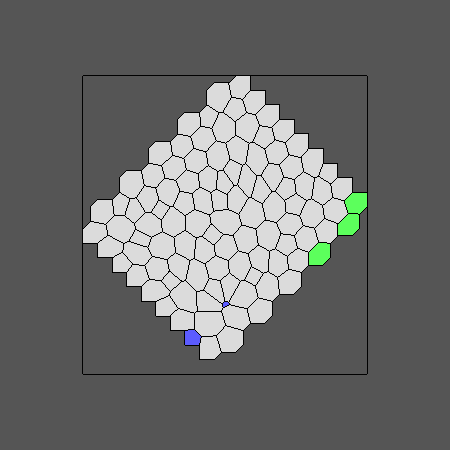
\includegraphics[width=0.5\textwidth]{../diagrams/rotate.png}
\caption{A Rotated Mesh for Error Analysis.}
\end{figure}

\chapter{The Future of \emph{Epithelium}}
\label{chap:advances}

We have thusfar explored the nature of epithelial tissue, discussed the variety of models that are currently in use, and thoroughly examined the \emph{Epithelium} implementation the Honda-Nagai Model. In this chapter, we will discuss some ideas for future epithelial tissue models. 

\begin{figure}[hb]
\centering
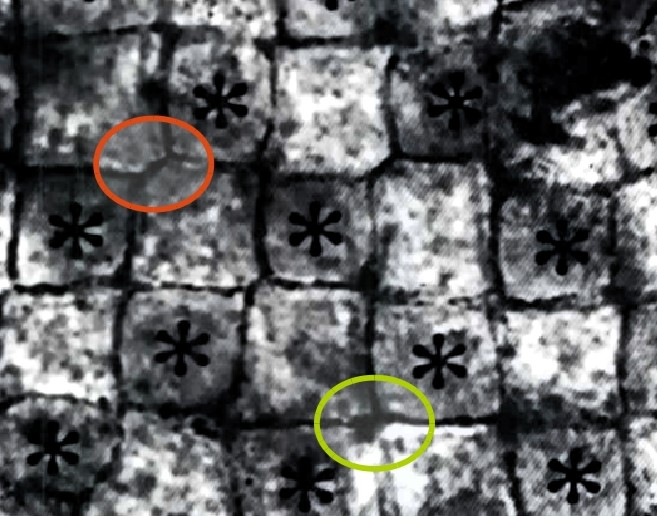
\includegraphics[width=0.5\textwidth]{../diagrams/checkers.jpg}
\caption{Square cells in quail epithelium. Image courtesy of~\cite{Checkers}.}
\label{fig:quail}
\end{figure}

\section{Rosette Models}
We have discussed the standard topology of epithelial tissue in great detail, but now we will explore a potential model with much different connectivity. Most models of epithelial tissue exclusively support vertices of degree three, but there is at least one tissue for which this topology may not be accurate. Figure~\ref{fig:quail} is taken from a paper by H. Yamanaka and H. Honda~\cite{Checkers} in which they model the dynamics of Japanese quail epithelium using exclusively degree three vertices. The fact is, however, that Figure~\ref{fig:quail} lends itself equally to interpretation as a mesh of degree four vertices or degree three vertices. It seems intuitively unlikely that the epithelial tissue of Japanese quails be the only tissue with this appearance, and a reasonable research idea is to find what other tissues have this property, and then subject meshes of this type to Honda-Nagai forces to see if the mesh remains a stable quadrilateral mesh as in nature. This type of experimentation could help resolve whether or not the Honda-Nagai Model is a good model for all types of tissue, or if it is strictly suited to tissues with predominantly six sided cells in equilibrium. In its current incarnation \emph{Epithelium} can only handle three cells meeting at a vertex, but more energy could be invested to make it handle different connectivities.

\section{A New Potential, A New Force}
In the Honda-Nagai Model, a harmonic form is given for the potential energies due to area and perimeter deformations, the gradient of which givens a hookean form\footnote{Hooke's law says that $F=-k\Delta x$.} for the force applied to a node (for more details, refer to~\ref{sec:force}). The assumptions underlying a model can render even the most seemingly accurate model physically meaningless if the assumptions are proven to be incorrect, and for this reason we should be skeptical about the harmonic formulation. In the literature the $C(x-x_0)^2$ form for the potential energy is asserted without biological evidence that it is correct, or even reasonable. Furthermore, assuming that cells are indeed elastic, there is no reason to believe that their elasticity fits the linear stress-strain curves prescribed by the hookean model.

There is a large class of materials including rubber and various elastomers that are classified as neo-hookean hyperelastic materials because their stress-strain\footnote{The stress-strain curve is the curve showing the amount of deformation(strain) in a material due to the application of varying amounts of force (stress).} curves are only linear in a small region (See Figure~\ref{fig:rubber}). After this region, the elasticity of the material becomes much higher~\cite{Rubber, Rubber2}. Hyperelastic models have been applied to various tissues with impressive results as in~\cite{hyperbio, hyperbio2}, but have only been briefly discussed with respect to epithelial tissue, as in~\cite{epihyper, epihyper2}.

The ideas of hyperelasticity need to be explored in more detail, and the conditions under which the Honda-Nagai elastic model is plausible ought to be better examined.

\section{Improvements in Imaging}
Another recent development in epithelial tissue science is the ability to record high quality videos of epithelial tissue during morphogenesis. One of the most impressive examples to date is the work being done in the Kiehart lab at Duke University where they are recording the closing of the epithelial envelope of \emph{Drosophila} embryos~\cite{Sokolow}. Through their recordings they have produced very good fits for certain modeling parameters and have performed an interesting experiment in which they try to keep the envelope from closing, but it closes anyway due to some currently unknown mechanism. 

\begin{wrapfigure}{r}{0.5\textwidth}
  \begin{center}
    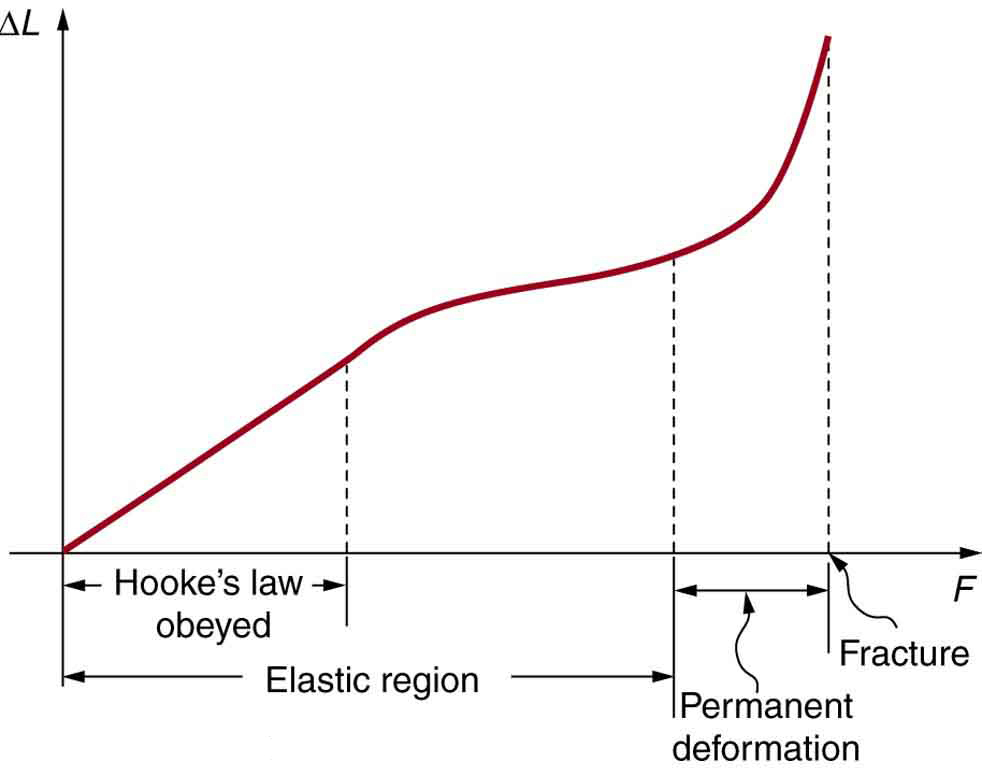
\includegraphics[width=0.48\textwidth]{../diagrams/rubber.jpeg}
  \end{center}
  \caption{The stress-strain curve for rubber. Image courtesy of~\cite{rubr}.}
\label{fig:rubber}
\end{wrapfigure}

An equally promising development in the field of epithelial tissue imaging is the work being done in the surface reconstruction of \emph{Drosophila} wings. Several softwares exist which can reconstruct a mesh of epithelial cells from an input image, but the most recent software released by L. Bai is able to take sets of images and faithfully reconstruct the apical face of a sheet of wing cells~\cite{3dwing}, even detecting 3D deformations. These imaging softwares will provide immense amounts of data about epithelial cell shapes and topology which will guide the development of future models, and perhaps serve as initial conditions and benchmarks for existing models. Unfortunately, the source code for the 3D imaging software is not freely available, and the possibility of developing an open source version ought to be considered. Very little is known about the accuracy of these softwares, as information about them comes exclusively from academic journal articles, and, depending on the quality of these imaging packages, competitive programs may be able to be developed in a short amount of time thanks to advanced libraries like Python's OpenCV~\cite{OpenCV}.

\section{Further Parallelization}
While the preceding ideas are very interesting and would contribute new ideas to the world of epithelial tissue modeling, the project of recreating the Honda-Nagai model was originally undertaken in the hopes of parallelizing the vast majority of the computations. Unfortunately, the trouble of efficiently storing a large tissue rendered the implementation of a parallel integrator seemingly impossible. 

The Chaste software is able to perform some computations in parallel, but only on the scale of a multi-core CPU, and not yet on the scale of a CUDA GPU~\cite{ChasteTutorial}. It is still possible to make a great contribution to the epithelial tissue community by discovering and sharing an effient datastructure and set of algorithms for storing and moving a sheet of epithelial cell vertices in parallel.

The first task in fully parallelizing the \emph{Epithelium}'s numerical integrations is storing the data in C arrays instead of classes, which will inevitably make the code's workings much more subtle than they currently are. Then, the next objective will be situating the data in an array in such that processors can effectively grab coalesced data chunks without too many expensive memory transactions. 

\section{Voronoi Tesselations}
The Honda-Nagai model \footnote{And other programs. The Voronoi Tesselation is one of the most famous algorithms in all of computational geometry. For more information see~\cite{tessel}} uses a periodic Voronoi Tesselation as the initial condition for the tissue~\cite{HondaNagai}, yet to the best of our knowledge an open source periodic Voronoi Tesselation program is unavailable. Indeed, the Voronoi Tesselation provides an ideal artificial initial mesh for an epithelial tissue simulation since all vertices have degree three and a careful choice of generating points can give all cells similar areas and perimeters. Several sources offer reliable software which computes a Voronoi Tesselation on the unbounded plane~\cite{boost, triangle}, while another freely available code performs the Voronoi Tesselation on 3D surfaces~\cite{voro++}, but none of these codes can perform the tesselation in a bounded box, or with periodic boundary conditions. 

The C++ Boost Library is a popular, heavily tested library for the C++ language, yet the Boost Voronoi Tesselation only computes the unbounded Voronoi Tesselation of a set of points, despite demand for a bounded Voronoi Tesselation as evidenced by questions~\cite{q1} on the programming website StackOverflow, and by the needs of epithelial modeling software. The lowest hanging fruit in the field of Voronoi Tesselations is the design of a bounding box algorithm for the Boost Voronoi Tesselation. A good second project would be to modify the Boost Voronoi functions so that they are able to produce periodic meshes. The expansion of this library would be a good service to modelers and to the C++ community in general.

\section{Visualization Software }
A final suggestion for the improvement of \emph{Epithelium}, and data presentation in general, is the development of an easy to use mesh visualization software which will take in data in a format similar to the OFF file format, and output an image of a mesh with highly customizable appearance. The vast majority of epithelial tissue simulations have rather bland graphical output, while others are very sharp and highly customizable. For examples of the current state of tissue visualization, see Figure~\ref{fig:fourgraphs}. 



\bibliographystyle{plain}
\bibliography{references}
\end{document}
